\chapter{Diseño e Implementación} \label{chap:analisisExperimentación}


\section{Diseño Pedagógico}

El diseño pedagógico se centra en el aprendizaje basado en problemas \cite{de2008aprendizaje}. Concretamente, se introduce la teoría relevante, que puede incluir explicaciones de texto, imágenes ilustrativas, y en ocasiones, material en formato de video. Una vez que el usuario ha absorbido el contenido teórico, se le presentan problemas prácticos relacionados para resolver.

Existen dos categorías principales de ejercicios, cada una con un peso distinto en la estructura de aprendizaje:

\begin {enumerate}
\item Ejercicios estándar: Son problemas prácticos que refuerzan la comprensión del usuario sobre el tema.

\item Ejercicios clave (\textit{key\_exercise}): Estos ejercicios desempeñan un papel crucial en la progresión del usuario. Son indicativos de si el usuario ha comprendido los requisitos fundamentales del tema en cuestión. Se deben completar estos ejercicios para avanzar al siguiente tema o módulo. Si el usuario no logra superar estos ejercicios en un primer intento, se le presentan ejercicios adicionales para reforzar su comprensión antes de volver a intentarlo.
\end{enumerate}

La plataforma corrige automáticamente para los módulos de C++, Java y Python, tal como se mencionó con anterioridad. Sin embargo, para el módulo de HTML+CSS+JS, se requiere una revisión manual por parte de un instructor. Esta revisión no solo califica el ejercicio, sino que también proporciona comentarios constructivos para guiar al usuario hacia la solución correcta.

Además de la corrección, la plataforma evalúa la limpieza y estructura del código presentado, ya que es esencial para un buen aprendizaje. Por lo tanto, se proporciona una retroalimentación detallada al estudiante no solo sobre la corrección de su respuesta, sino también sobre cómo mejorar y optimizar su código.

Finalmente, la plataforma tiene la capacidad de compilar ejercicios, permitiendo la verificación y corrección del código antes de su envío.

\subsection{Gamificación}

La gamificación en el contexto educativo se incorpora con el fin de mejorar la motivación y el compromiso de los estudiantes. Al completar un módulo, se desbloquea un juego específico que el estudiante debe adquirir una sola vez, y luego tendrá acceso ilimitado a él. Esta estrategia se alinea con teorías motivacionales y de refuerzo positivo, proponiendo un equilibrio entre el aprendizaje serio y la diversión. La elección de estos juegos no ha sido aleatoria; cada uno ha sido seleccionado por su potencial para desarrollar habilidades cognitivas que son transferibles al dominio de la programación. Concretamente, la selección de juegos ha sido:

\begin{itemize}
    \item \textbf{Buscaminas:} Clásico juego de resolución de problemas que mejora la atención al detalle y el análisis lógico.
    
    \item \textbf{2048:} Este es un juego de lógica y estrategia numérica que fomenta el pensamiento crítico y la planificación anticipada, habilidades muy útiles en la programación.
    
    \item \textbf{Hextris:} Juego que exige una rápida toma de decisiones y mejora la agilidad mental, promoviendo una mejor respuesta bajo presión, una situación común en la depuración de código.
    
    \item \textbf{Ajedrez:} Conocido por desarrollar habilidades estratégicas, el ajedrez también enseña a los estudiantes a pensar en términos de múltiples posibilidades y consecuencias, similar a la elaboración de algoritmos en la programación.
\end{itemize}

Al requerir que los estudiantes paguen por el juego (utilizando puntos que ganan al completar ejercicios), se añade un sentido de valor y recompensa por el esfuerzo realizado en el aprendizaje. Esta mecánica de  \textit{pago por recompensa} también simula un entorno real donde las recompensas se ganan a través del esfuerzo y el logro.

Además, la gamificación actúa como un sistema de descanso entre sesiones de estudio intensivas, lo que puede ayudar a prevenir la fatiga mental y a mantener la mente de los estudiantes fresca y enfocada. Estudios han demostrado que los descansos estructurados pueden mejorar la productividad y la creatividad, aspectos fundamentales para un aprendizaje efectivo y sostenido \cite{ariga2011brief}.

La implementación de la gamificación en la plataforma se ha realizado con cuidado para asegurar que los juegos sirvan como un complemento al material educativo y no como una distracción. Es un balance delicado que se busca manejar para enriquecer la experiencia de aprendizaje global.

\section{Arquitectura del Sistema}

La interacción del usuario en el Frontend se lleva a cabo utilizando tecnologías estándar como HTML sin emplear \textit{frameworks} adicionales para su desarrollo. Además, la interfaz es \textit{Web Responsive}, lo que garantiza su adaptación a variados dispositivos. Desde el punto de vista de la seguridad, se han implementado medidas como la validación de entradas, previniendo así amenazas como los ataques XSS. Los datos de sesión se conservan en el cliente mediante cookies.

Por otro lado, el Backend se ha desarrollado con Flask. Se encarga de administrar las API RESTful y de establecer una conexión ininterrumpida con la base de datos PostgreSQL. La biblioteca \textit{flask\_login} respalda las funcionalidades de autenticación y autorización, aportando una capa de seguridad adicional. La lógica de negocio del sistema reside principalmente en el Sistema de Tutoría Inteligente (ITS). Este subsistema es el encargado de la elección y evaluación de ejercicios, ofreciendo retroalimentación y monitoreando el avance del estudiante.

\begin{figure}[H]
    \centering
    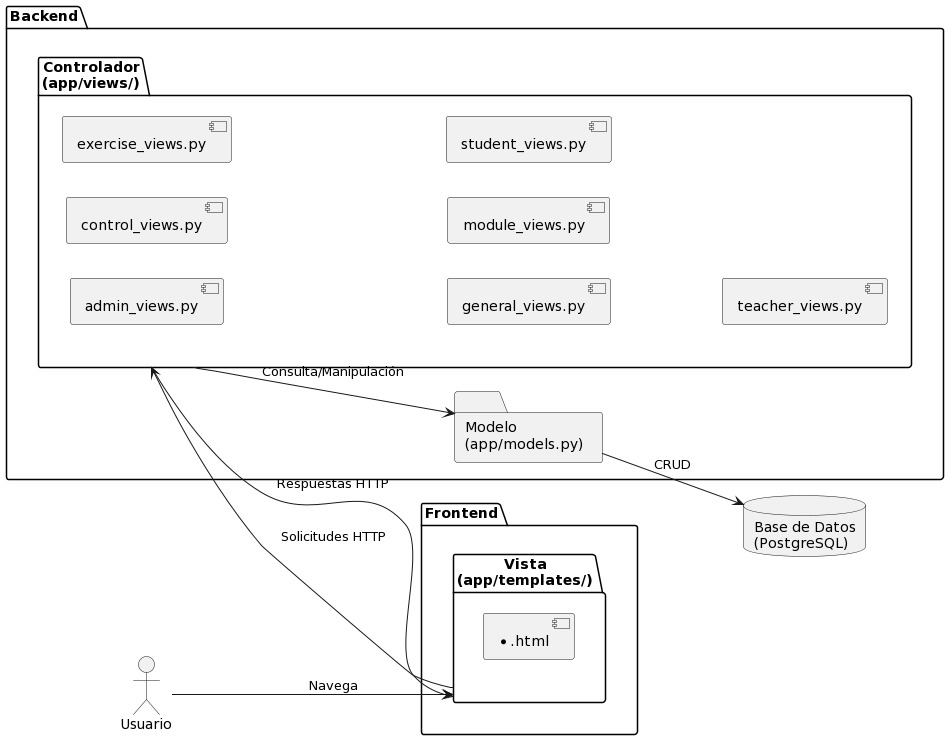
\includegraphics[width=0.7\textwidth]{imagenes/ArquitecturaDeSistema.jpeg}
    
    \caption{Arquitectura de sistema}
    \label{fig:arqsistema}
\end{figure}

En relación con la seguridad del Backend, se han establecido roles y restricciones de acceso coherentes con las reglas de negocio previamente determinadas. Aunque la arquitectura actual no posee herramientas concretas orientadas a la escalabilidad, está concebida para ser resistente y estable.

Es esencial destacar que, la estructura general del sistema sigue el patrón Modelo-Vista-Controlador (MVC). La Vista reside en el Frontend, y el Controlador y Modelo en el Backend \ref{fig:arqsistema}. Este patrón facilita la distinción entre la lógica de la interfaz de usuario y las operaciones, simplificando su mantenimiento.

\section{Diseño de Base de Datos}

La arquitectura de nuestra base de datos es el resultado de un exhaustivo análisis y diseño. Su estructura no solo atiende a las necesidades actuales, sino que también se anticipa a los retos futuros. A continuación, detallamos algunos de los elementos clave y las consideraciones adoptadas en su construcción:

\begin{enumerate}
    \item \textbf{Tablas principales y su significado}: Las tablas como \textit{users}, \textit{modules}, \textit{requirements}, \textit{exercises}, \textit{questions} y \textit{theory} son la columna vertebral de la base de datos. En ellas, se almacena la información medular que alimenta las funcionalidades centrales del sistema. Estas tablas, además de contener datos primordiales, están interconectadas a través de relaciones específicas. Garantizando, así, la coherencia y la integridad de la información en todo momento.
    
    \item  \textbf{La importancia de los índices}: Los índices son herramientas fundamentales para acelerar las consultas y garantizar un rendimiento óptimo. Dentro de la base de datos, su uso es estratégico. Existen índices únicos, como el \textit{users\_email\_key}, que aseguran la singularidad de ciertos registros. Por ejemplo, en el caso del correo electrónico, se garantiza que no existan duplicados. Los índices compuestos, como \textit{student\_modules\_student\_id\_module\_id\_key}, son esenciales para optimizar las consultas que abarcan múltiples campos. Las tablas intermedias, que representan relaciones entre otras, también hacen uso de índices. En este caso, \textit{exerciserequirements} y \textit{theoryrequirements}. Estos índices, principalmente compuestos, agilizan y refuerzan las consultas relacionales.

    \item \textbf{La normalización como estándar}: Uno de los principios fundamentales que se ha seguido es la normalización. Al estructurar la información de esta manera, se minimiza la redundancia y maximiza la eficiencia.

    \item \textbf{Relaciones bien definidas}: La claridad en las relaciones entre tablas es esencial. Gracias a las claves primarias y foráneas, se ha conseguido una red de relaciones que no solo facilita la integración y consulta de datos sino que también refuerza la integridad de los mismos.

    \item \textbf{Mirando hacia el futuro}: Más allá de las necesidades actuales, el diseño busca ser resiliente y adaptable. Pretendiendo que cualquier adición futura, ya sea en funcionalidades o módulos, se integre sin grandes complicaciones.
\end {enumerate}


Por ello, la base de datos del sistema es robusta, detallada y diseñada para crecer. Teniendo como aspiración que, más allá de ser un simple almacén de datos, sea una herramienta eficiente que potencie la experiencia del usuario y facilite el trabajo de la ITS.

\newpage

\begin{figure}[H]
    \centering
    \begin{sideways}
        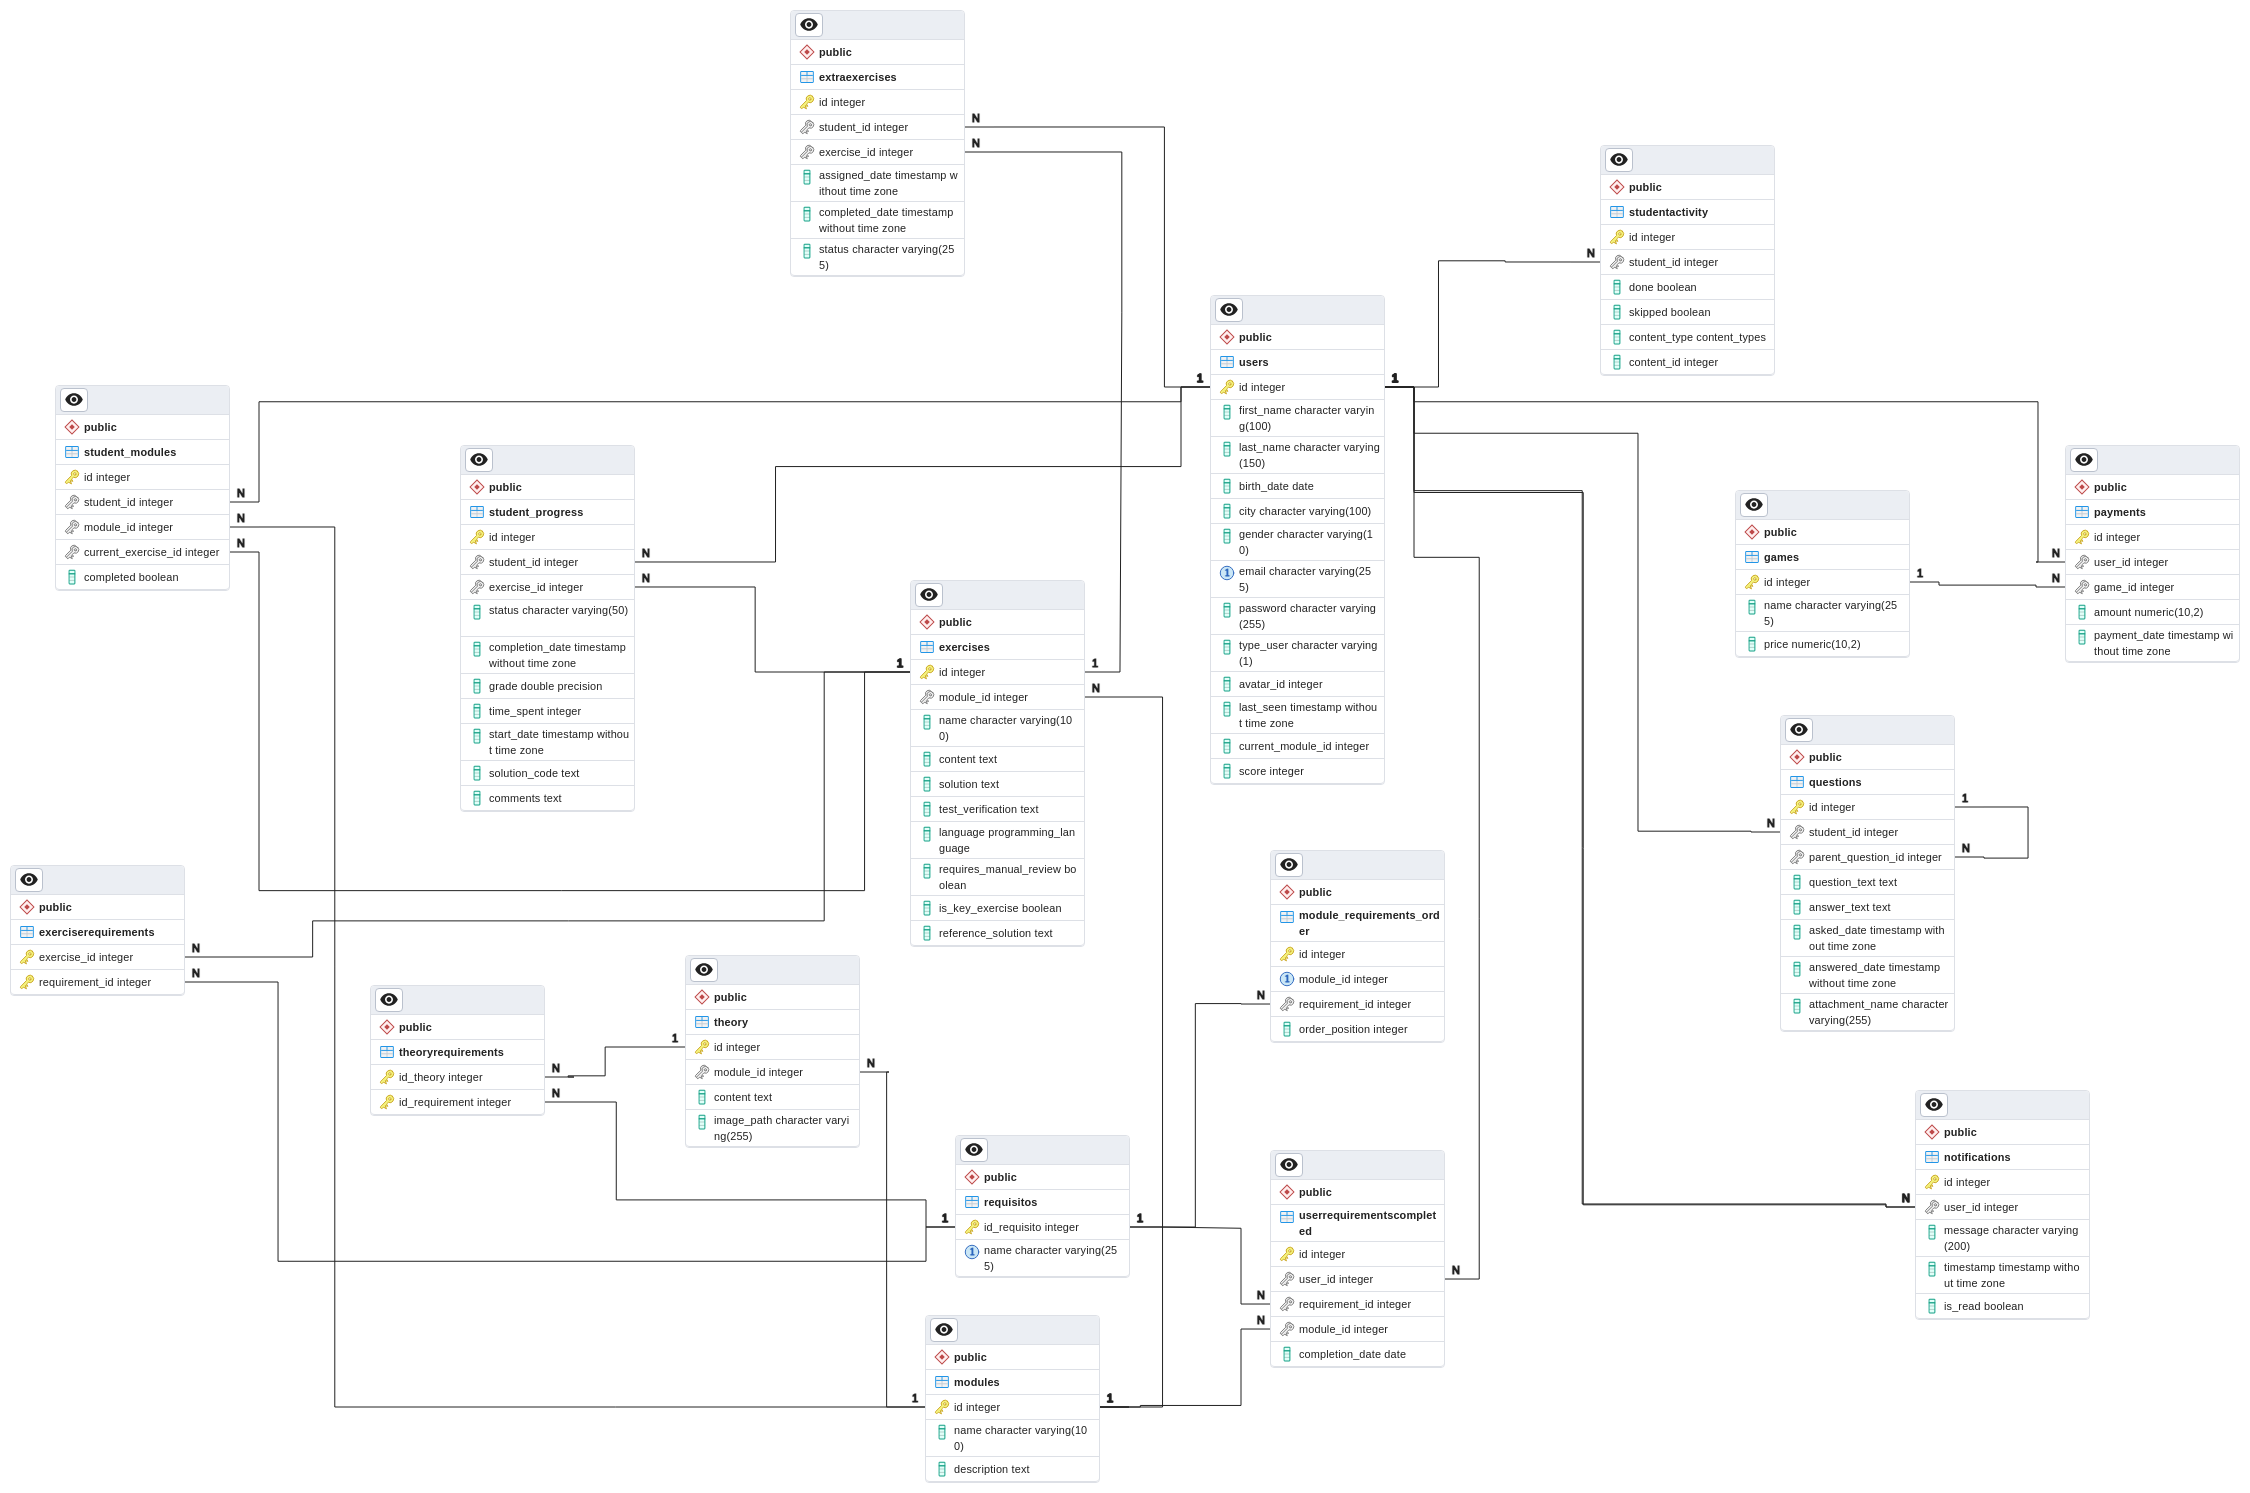
\includegraphics[width=1.8\textwidth]{imagenes/er.png}
    \end{sideways}
    \caption{Diagrama del modelo de datos}
    \label{fig:modeladodedatos}
\end{figure}

\section{Interfaz de Usuario}


\subsection{Interacción Usuario-Sistema}

El sistema está diseñado para una comunicación efectiva y amigable con el usuario. La fluidez en la navegación y la clara representación de opciones forman una experiencia de usuario destacable.

\begin{enumerate}
    \item \textbf{Inicio de Sesión}: Al entrar, la primera pantalla es la de inicio de sesión. Aquí, el usuario introduce su nombre y contraseña. Si las credenciales son correctas, se redirige a la página principal. De lo contrario, un breve mensaje de error informa del problema.
    
    \item \textbf{Registro}: Para nuevos usuarios, hay una pantalla especial donde se pide la información básica.
    
    \item \textbf{Página Principal}: Una vez dentro, la página principal se despliega. Ofrece múltiples funciones: desde juegos hasta rankings. Iconos y etiquetas guían al usuario, haciendo la navegación intuitiva.
    
    \item \textbf{Juegos, Teoría y Ejercicios}: Estas secciones son el corazón educativo del sistema. Los juegos son la motivación del estudiante. La teoría ofrece contenido educativo valioso y los ejercicios proponen retos prácticos que evalúan el aprendizaje del usuario.
    
    \item \textbf{Contacto con el profesor y Ranking}: Dos secciones cruciales. En 'Contacto con el profesor', el usuario puede realizar consultas y ver sus anteriores dudas conjuntamente con los comentarios de algunos ejercicios. 'Ranking' motiva a los usuarios mostrando una lista de los más destacados.
    
    \item \textbf{Interfaz del Profesor}: No solo los estudiantes tienen espacio en el sistema. Los profesores tienen su propia interfaz. Pueden observar estadísticas, corregir tareas y más. También tienen acceso a un panel administrativo.
    
    \item \textbf{Notificaciones}: Finalmente, las notificaciones juegan un papel vital. Informan al usuario sobre correcciones, nuevos contenidos o interacciones. Esta comunicación directa asegura que el usuario esté siempre al tanto de los eventos relevantes.
\end{enumerate}

El \textbf{Panel del Administrador} es una herramienta esencial para la gestión de la base de datos. Concretamente, ofrece una interfaz gráfica que evita la necesidad de interactuar a través de la terminal. Este enfoque agiliza las tareas cotidianas, y reduce la posibilidad de errores humanos que podrían surgir al gestionar datos de forma manual. Es importante mencionar que solo hemos mostrado un contexto general de la interfaz dentro de los mockups presentados. Estas representaciones cubren las funciones básicas, por ello, incluir más detalles sería redundante, ya que las operaciones fundamentales están claramente ilustradas.

En resumen, el sistema busca una interacción amena y productiva proporcionando las herramientas que necesitan los diferentes usuarios, presentadas de manera clara y accesible.

\subsection{\textit{Mockups} de la página web}

Este apartado incluye una serie de \textit{mockups} que representan las diferentes interfaces de usuario del sistema. Los \textit{mockups} han sido diseñados utilizando la herramienta en línea \textit{wireframe.cc} \cite{wireframe}. Esta herramienta permite la creación rápida y eficiente de prototipos de interfaces, facilitando la visualización y el diseño preliminar de las interacciones del usuario que se muestran a continuación.

\begin{figure}[H]
    \centering
    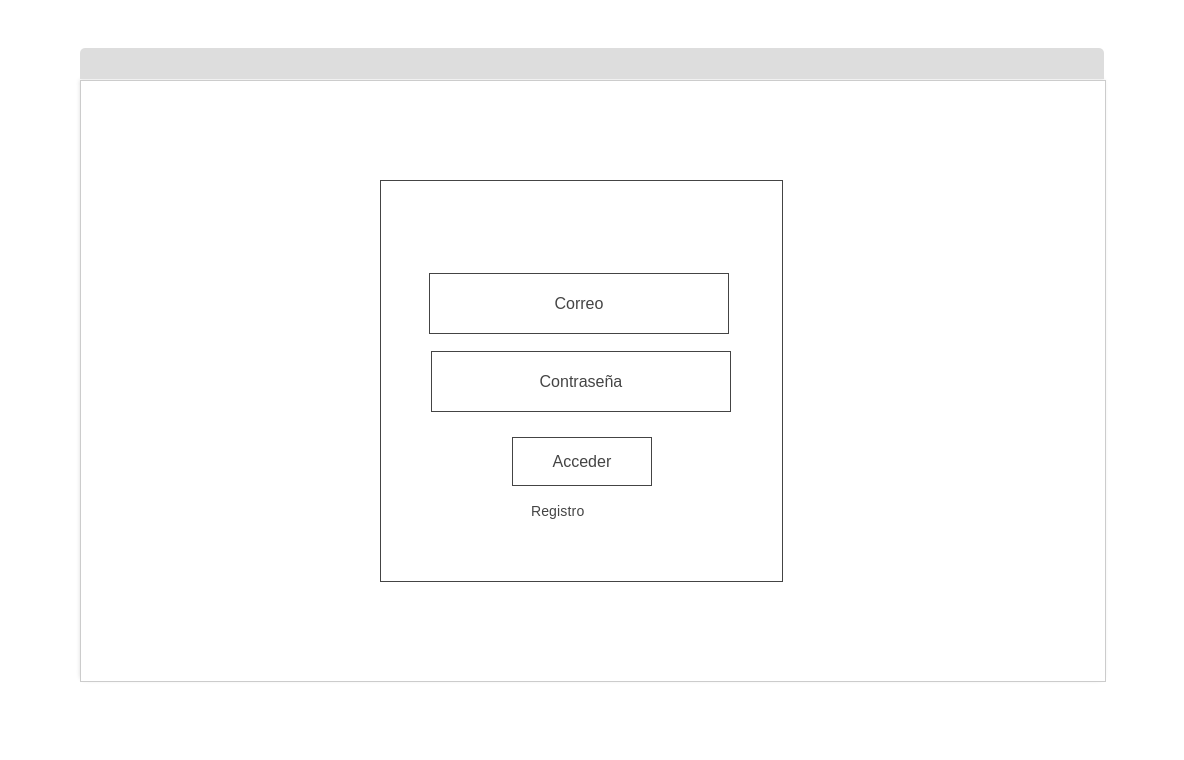
\includegraphics[width=0.6\textwidth]{imagenes/Mockups/1-InicioDeSesion.png}
    \caption{Inicio de Sesión para cualquier usuario.}
\end{figure}

\begin{figure}[H]
    \centering
    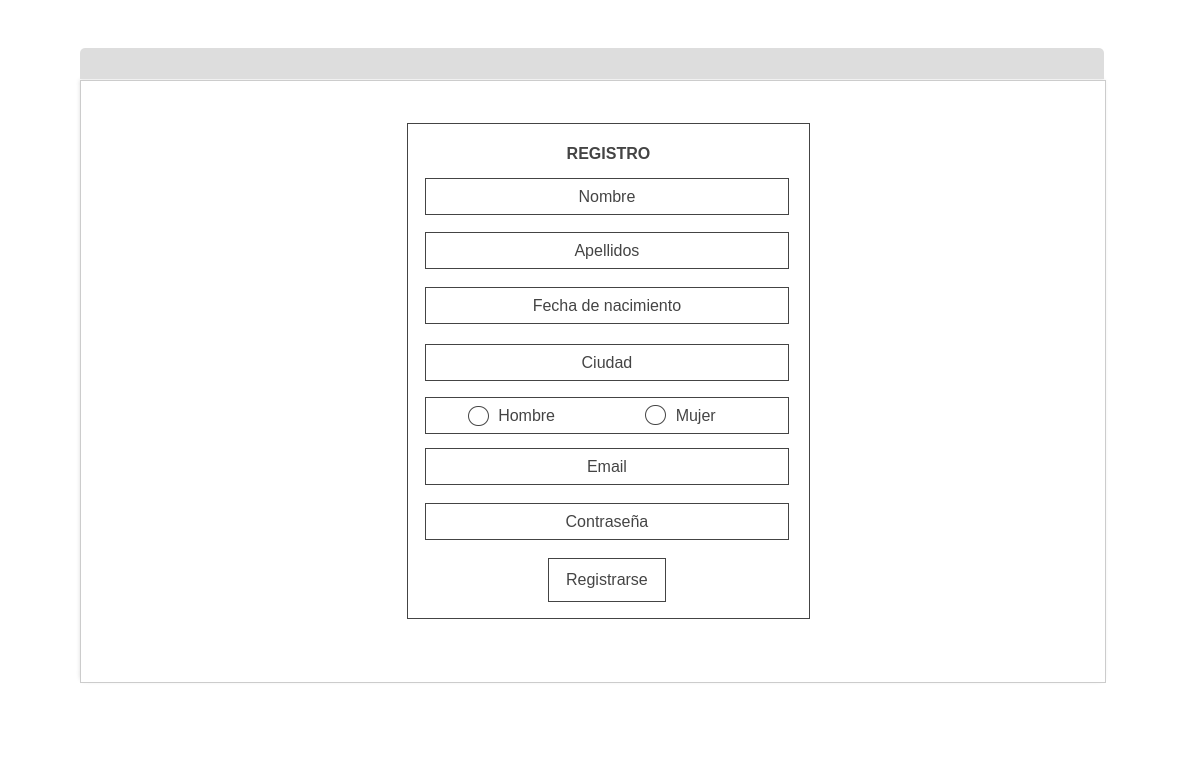
\includegraphics[width=0.6\textwidth]{imagenes/Mockups/2-Registro.png}
    \caption{Registro para cualquier usuario.}
\end{figure}

\begin{figure}[H]
    \centering
    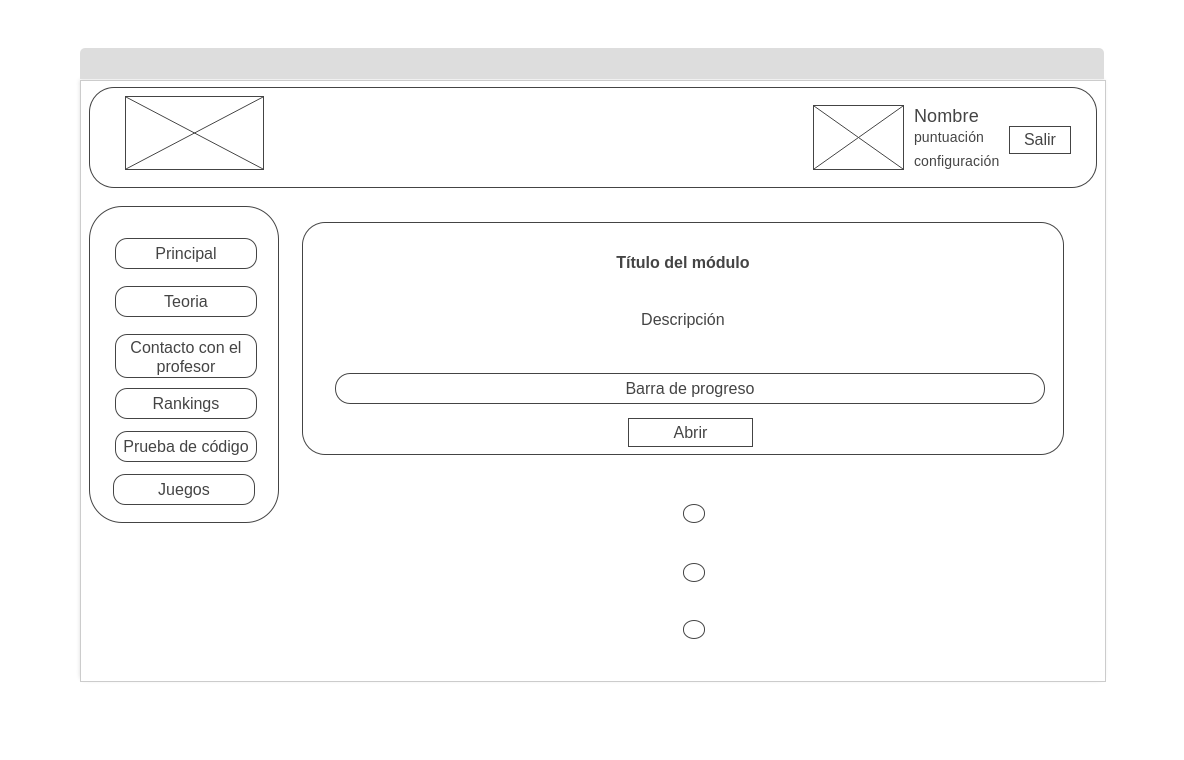
\includegraphics[width=0.6\textwidth]{imagenes/Mockups/3-Pag-Principal.png}
    \caption{Página Principal  de la interfaz del estudiante.}
\end{figure}

\begin{figure}[H]
    \centering
    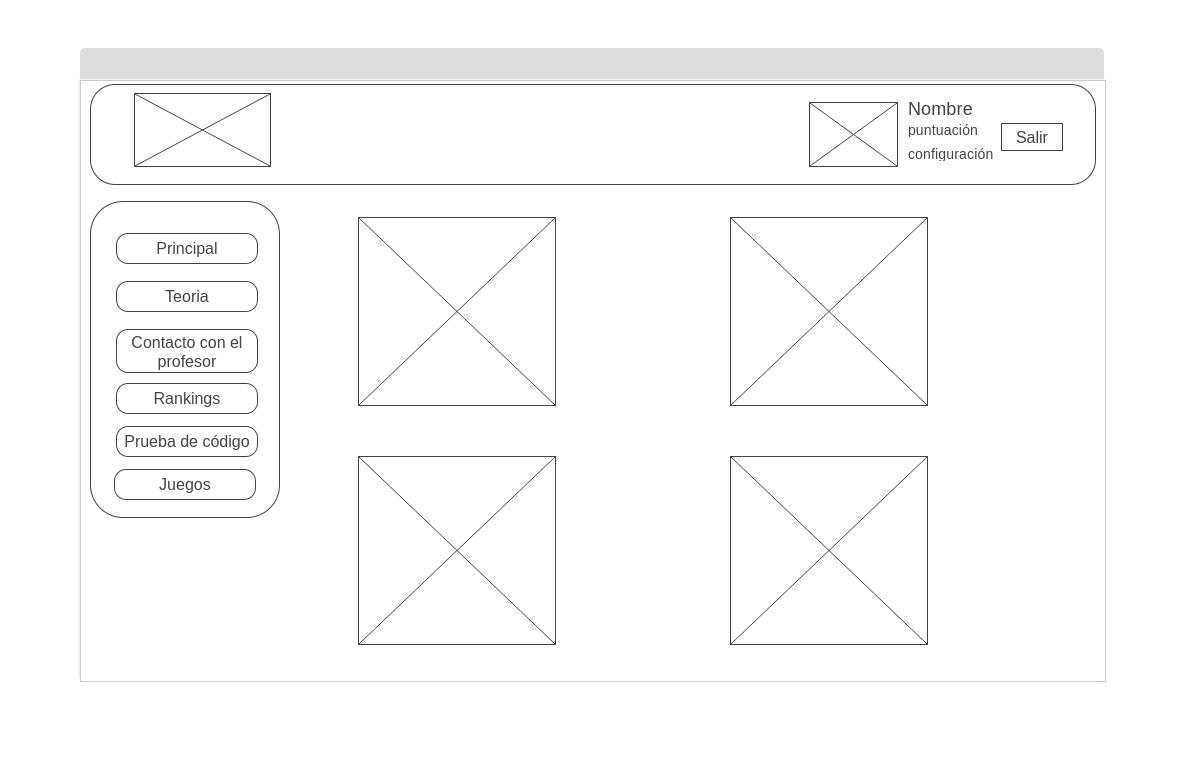
\includegraphics[width=0.6\textwidth]{imagenes/Mockups/4-Juegos.png}
    \caption{Apartado de Juegos de la interfaz del alumno.}
\end{figure}

\begin{figure}[H]
    \centering
    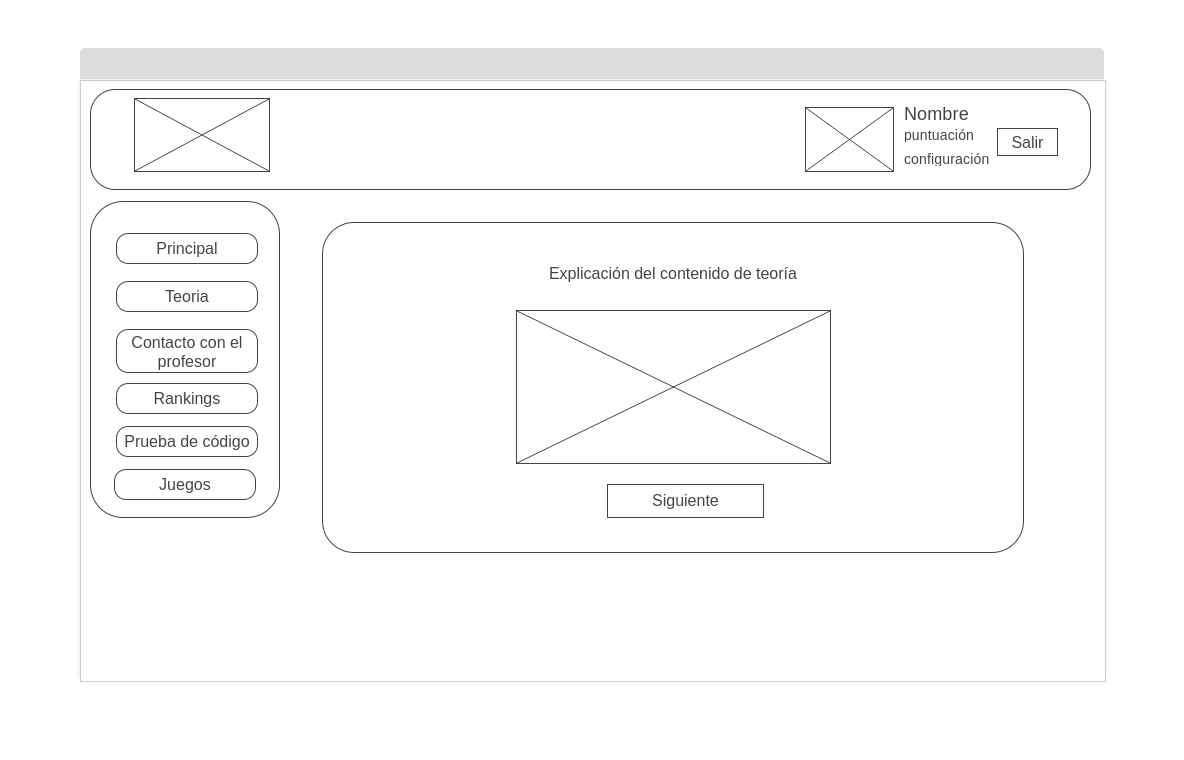
\includegraphics[width=0.6\textwidth]{imagenes/Mockups/5-Teoria.png}
    \caption{Visualización de la teoría para el estudiante.}
\end{figure}

\begin{figure}[H]
    \centering
    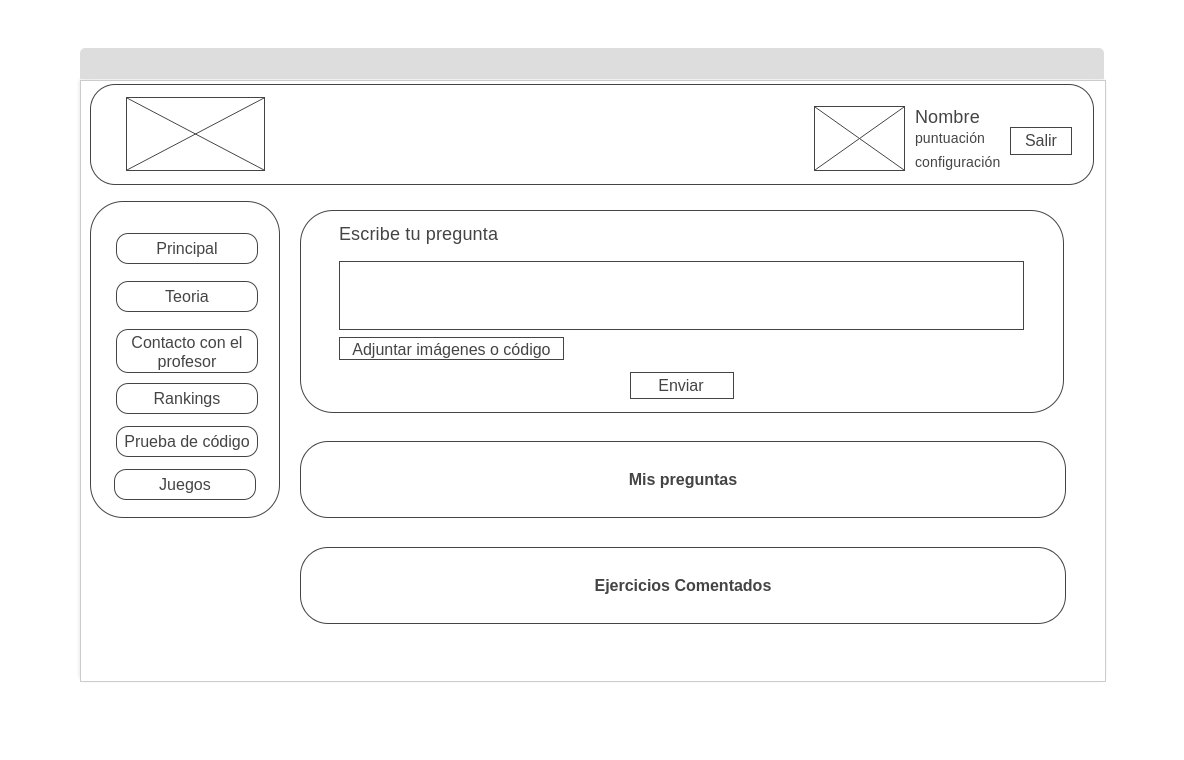
\includegraphics[width=0.6\textwidth]{imagenes/Mockups/6-Consulta.png}
    \caption{Apartado de contacto con el profesor.}
\end{figure}

\begin{figure}[H]
    \centering
    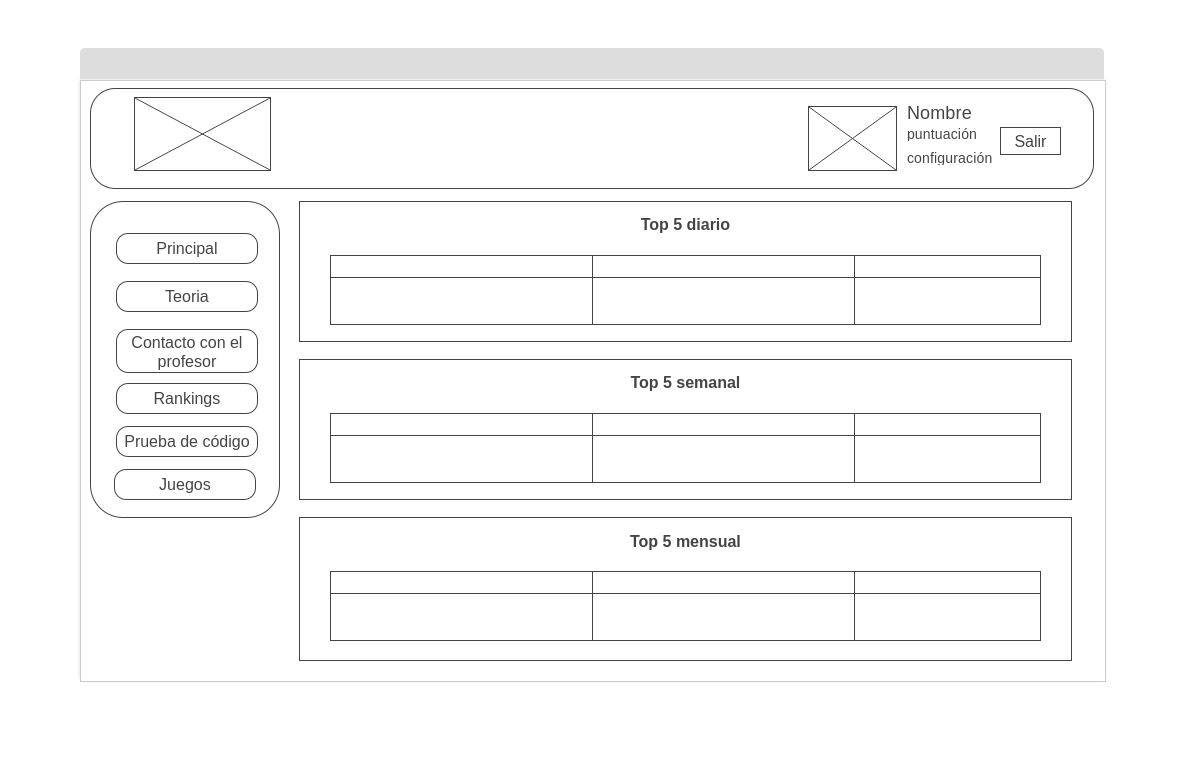
\includegraphics[width=0.6\textwidth]{imagenes/Mockups/7-Ranking.png}
    \caption{Apartado de Ranking de la interfaz del usuario.}
\end{figure}


\begin{figure}[H]
    \centering
    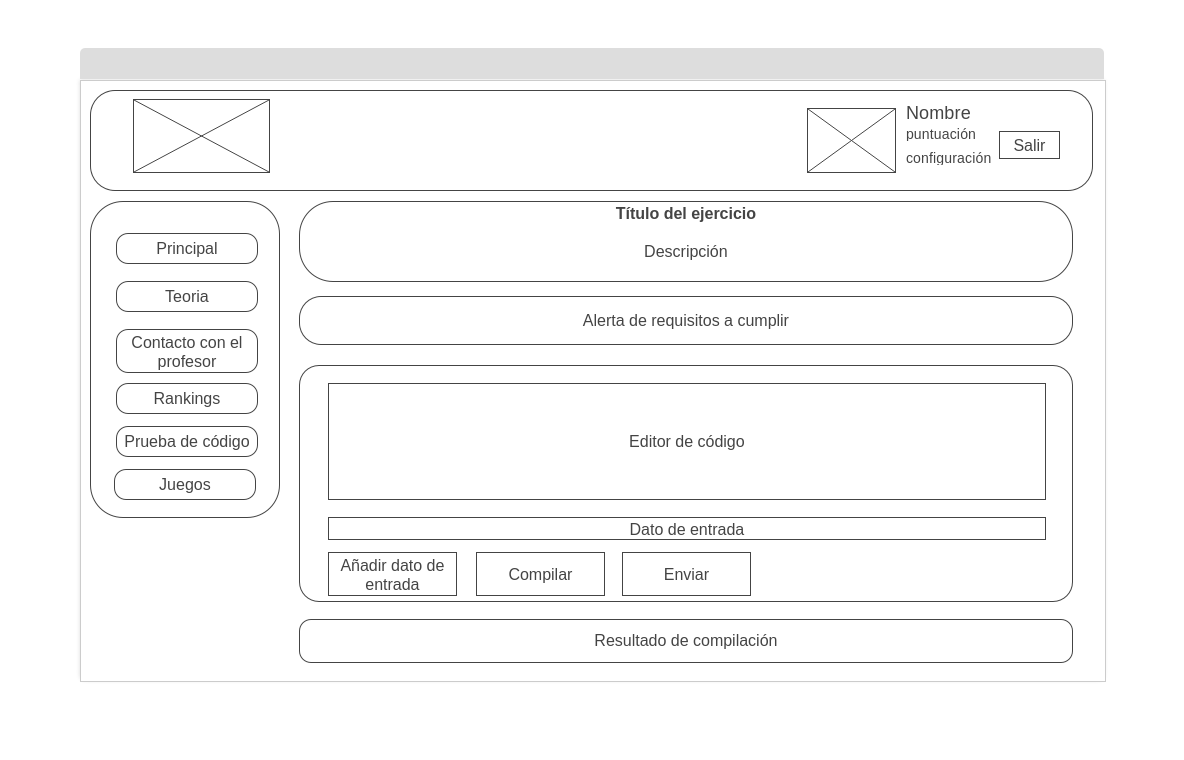
\includegraphics[width=0.6\textwidth]{imagenes/Mockups/8-Ejercicio.png}
    \caption{Visualización de los ejercicios para el usuario.}
\end{figure}

\begin{figure}[H]
    \centering
    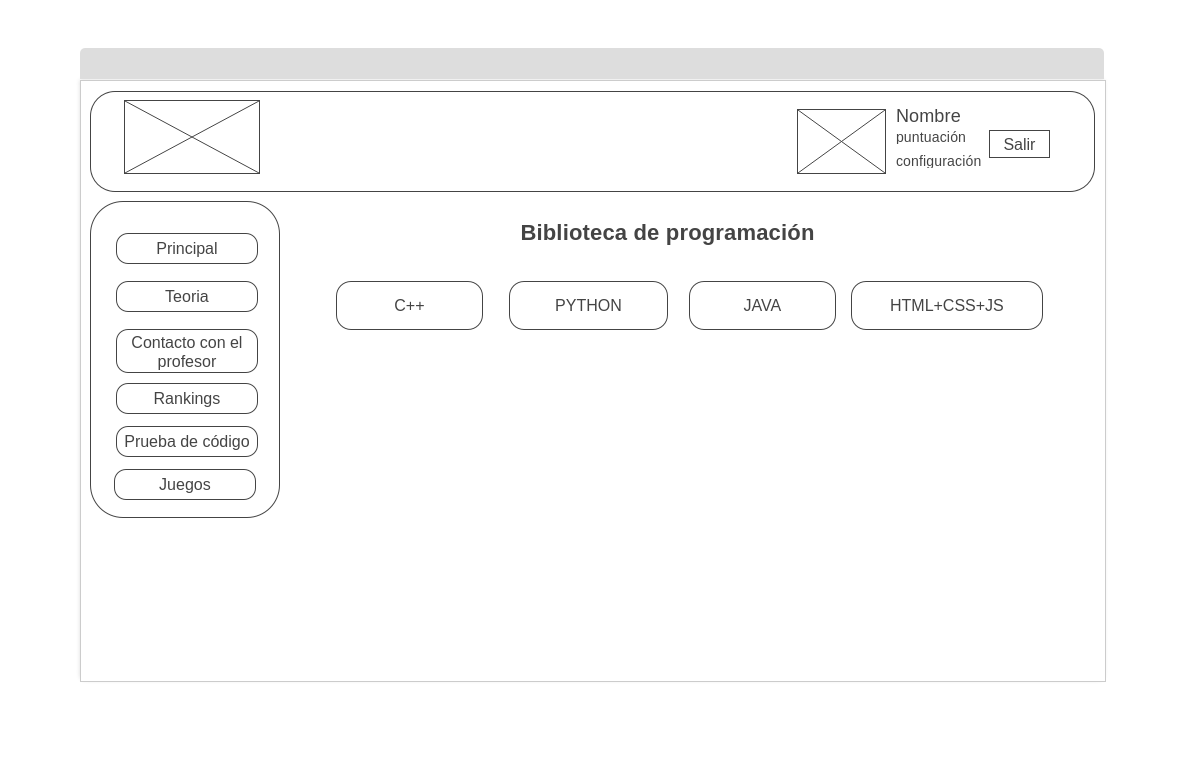
\includegraphics[width=0.6\textwidth]{imagenes/Mockups/9-Consulta-Teoria.png}
    \caption{Apartado donde los estudiantes pueden revisar conceptos teóricos.}
\end{figure}

\begin{figure}[H]
    \centering
    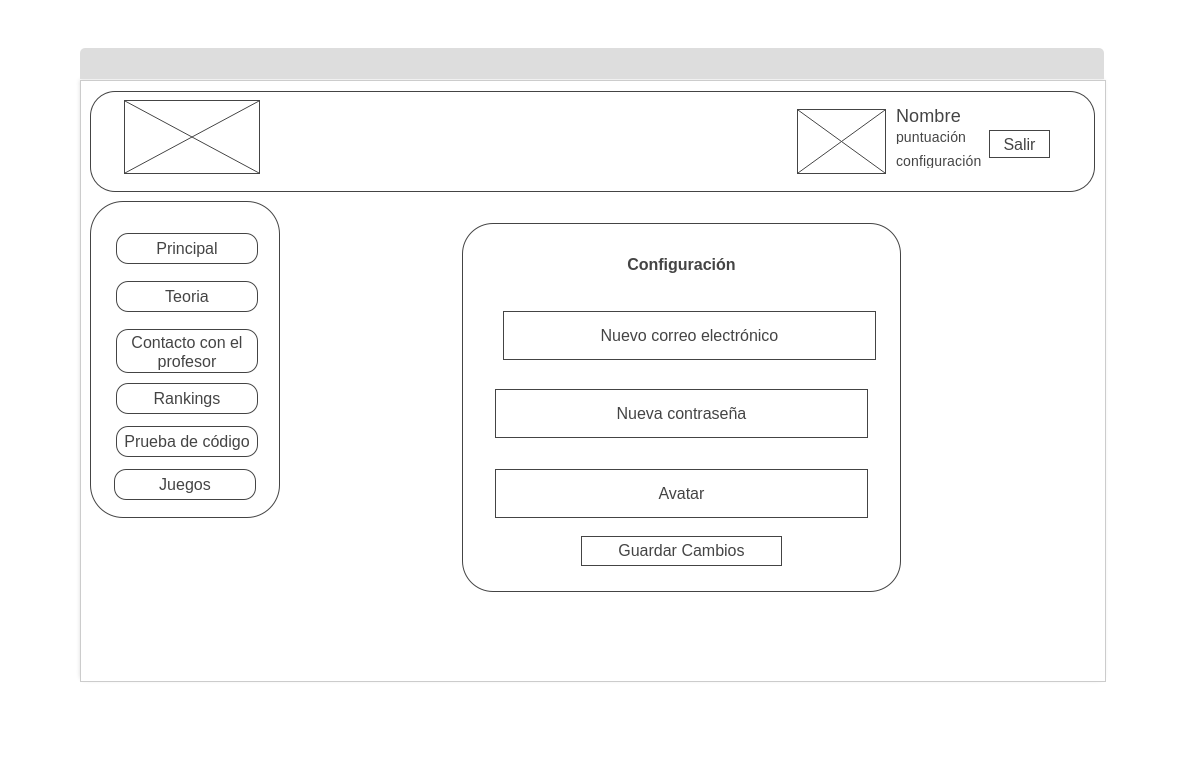
\includegraphics[width=0.6\textwidth]{imagenes/Mockups/10-Configuracion-Est-.png}
    \caption{Apartado de configuración del estudiante.}
\end{figure}

\begin{figure}[H]
    \centering
    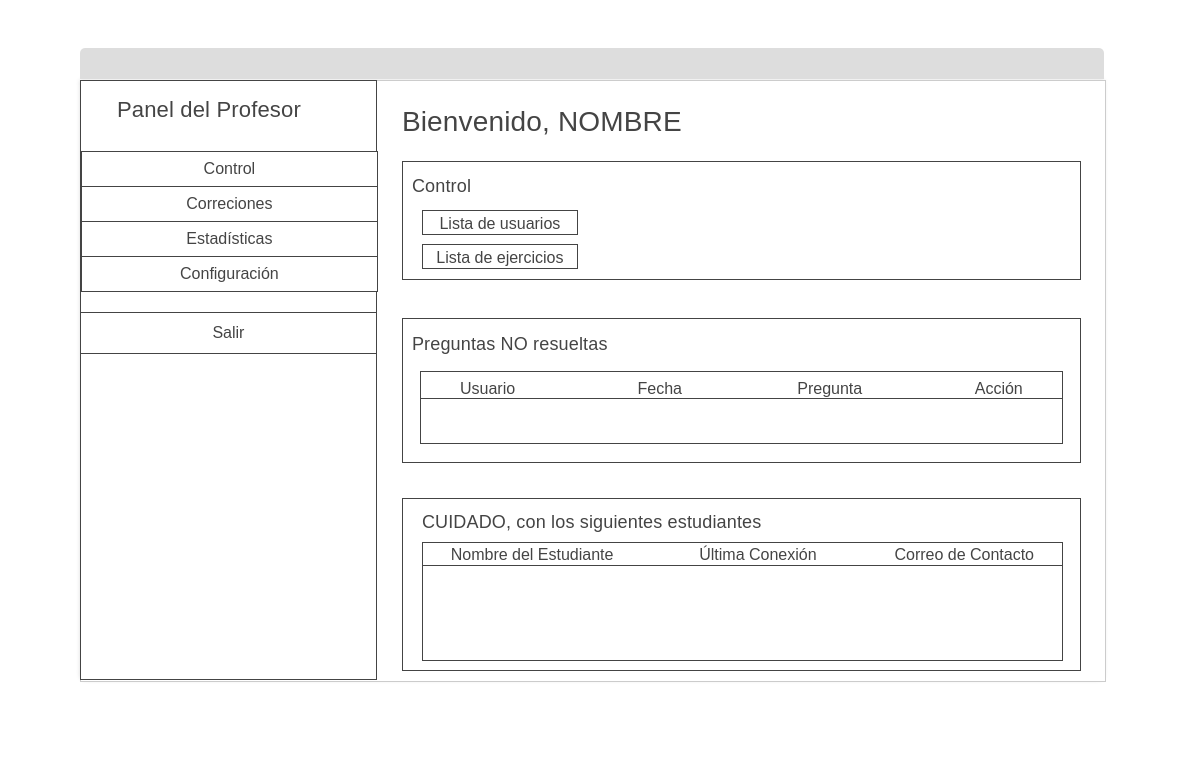
\includegraphics[width=0.6\textwidth]{imagenes/Mockups/11-Profesor-Principal.png}
    \caption{Dashboard principal del profesor.}
\end{figure}

\begin{figure}[H]
    \centering
    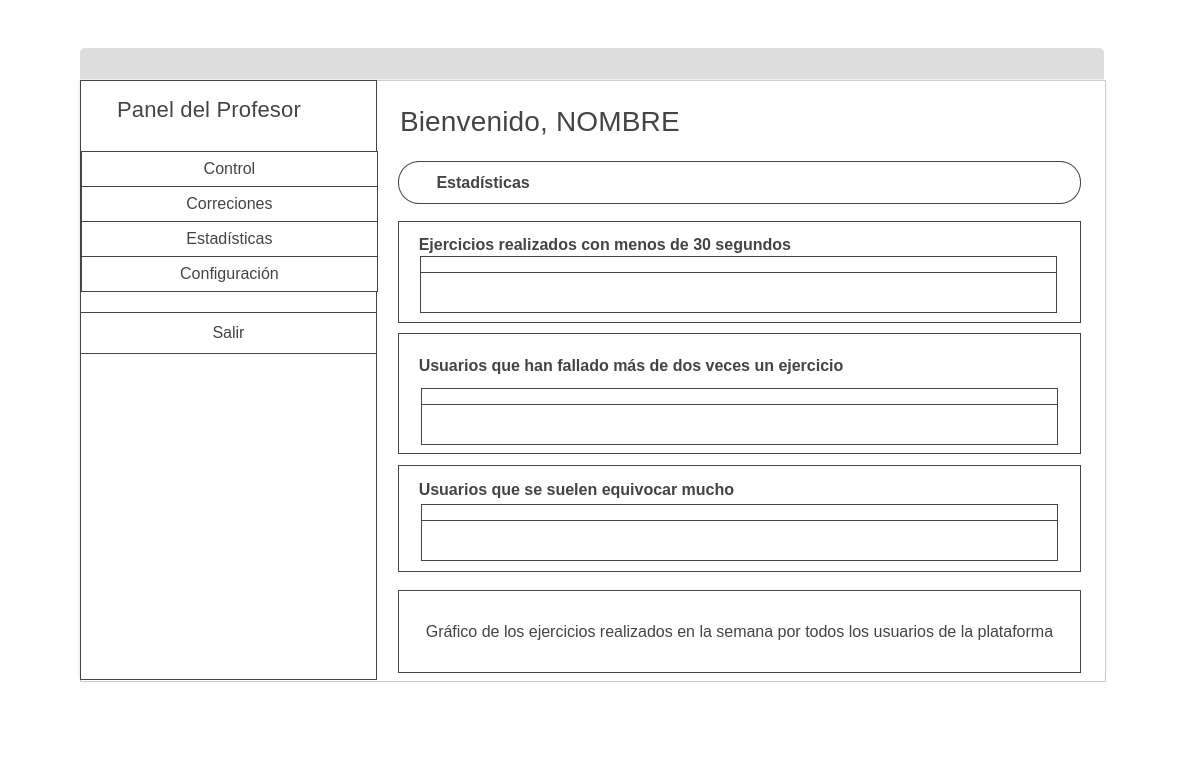
\includegraphics[width=0.6\textwidth]{imagenes/Mockups/12-Profesor-Estadisticas.png}
    \caption{Pantalla de Estadísticas del profesor.}
\end{figure}

\begin{figure}[H]
    \centering
    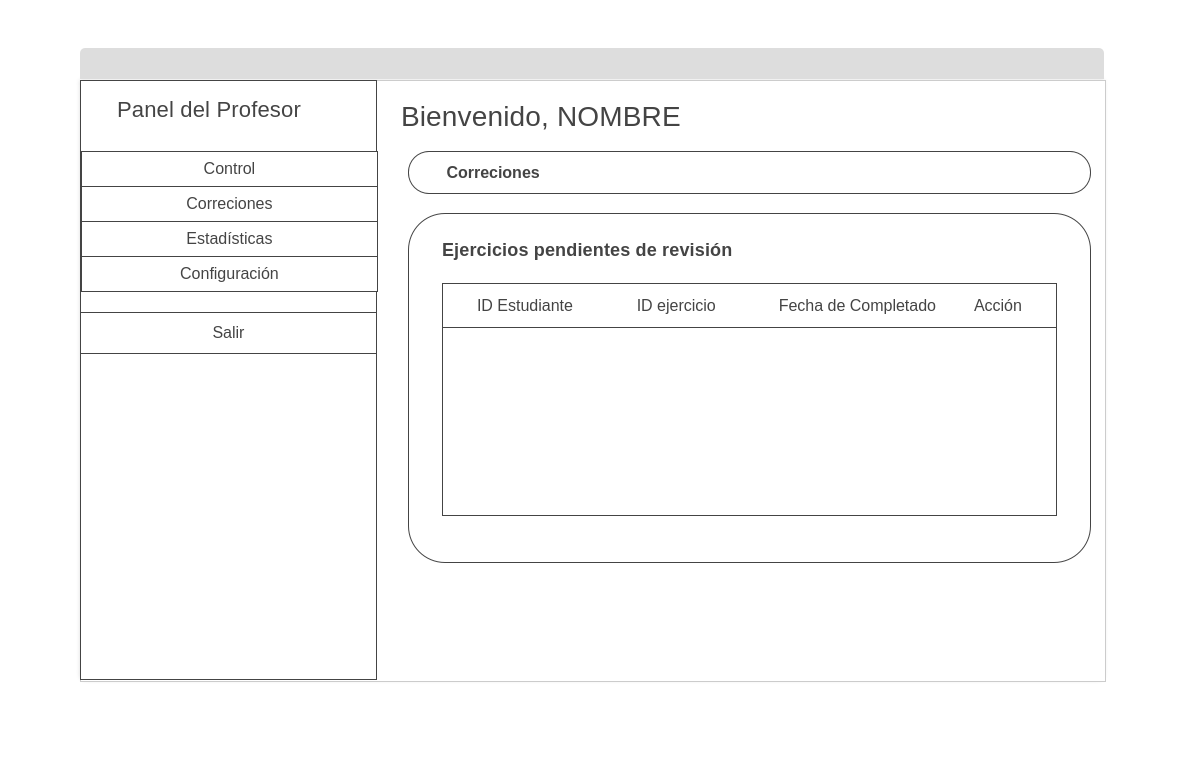
\includegraphics[width=0.6\textwidth]{imagenes/Mockups/13-Profesor-Corregir.png}
    \caption{Pantalla con la lista de corrección de ejercicios.}
\end{figure}

\begin{figure}[H]
    \centering
    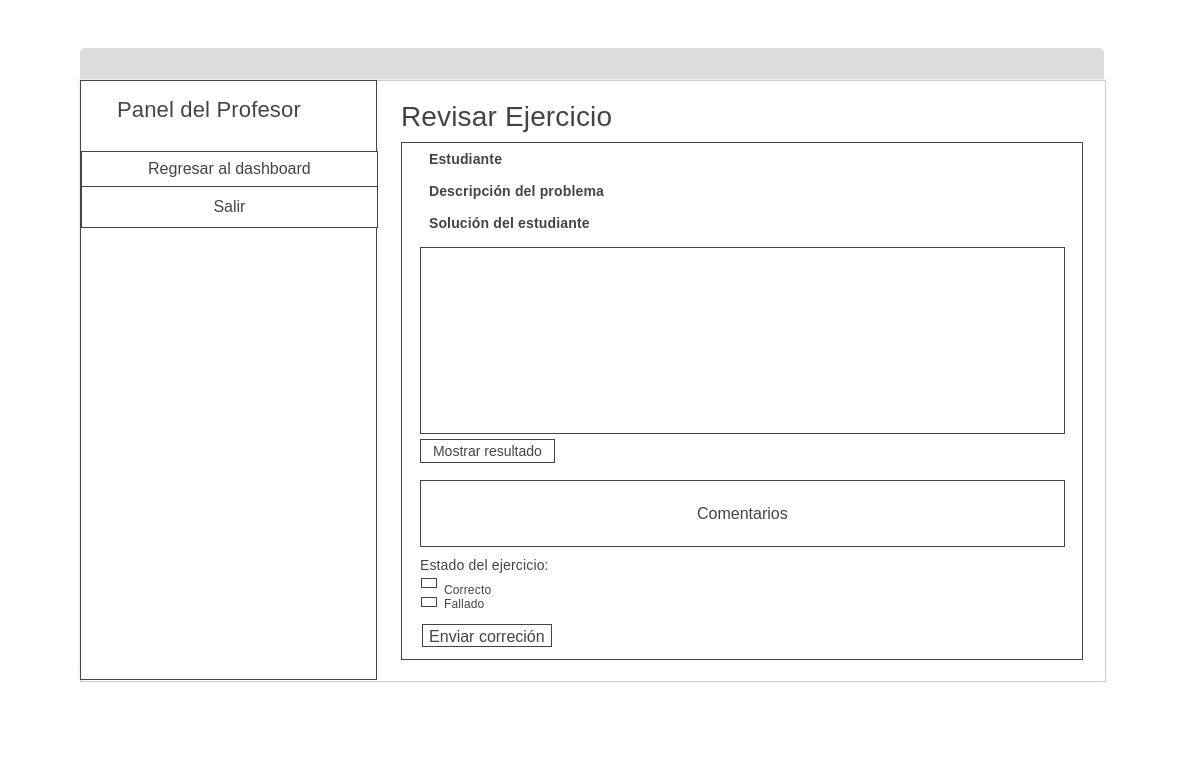
\includegraphics[width=0.6\textwidth]{imagenes/Mockups/14-Profesor-Corregir-Ejercicio.png}
    \caption{Panel para facilitar la corrección los ejercicios para el profesor.}
\end{figure}

\begin{figure}[H]
    \centering
    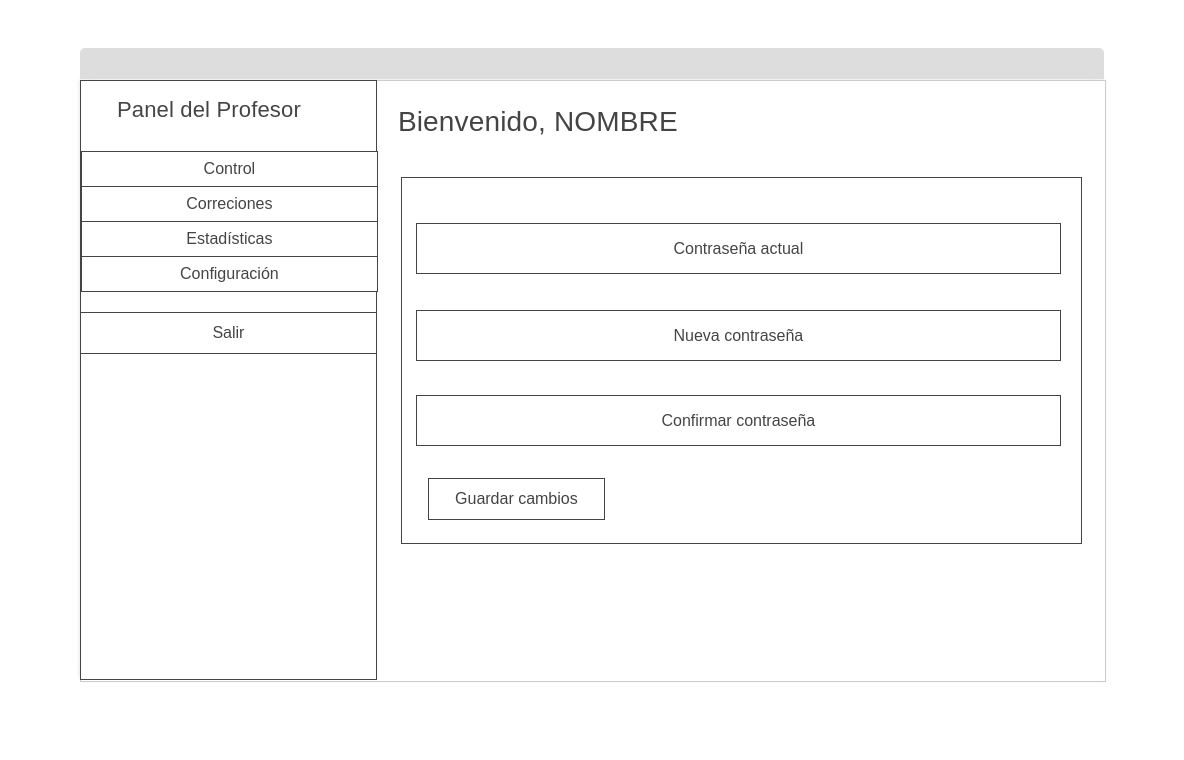
\includegraphics[width=0.6\textwidth]{imagenes/Mockups/15-Profesor-Configuracion.png}
    \caption{Apartado de Configuración del profesor.}
\end{figure}

\begin{figure}[H]
    \centering
    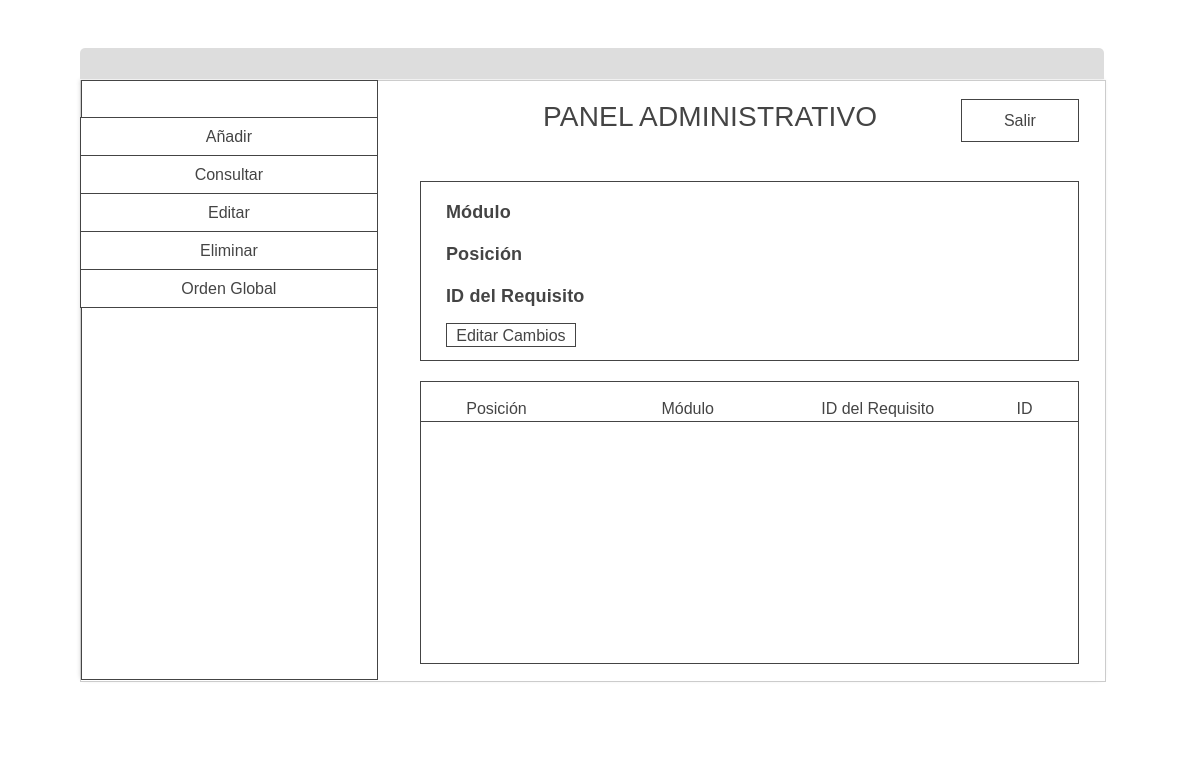
\includegraphics[width=0.6\textwidth]{imagenes/Mockups/16-Panel-Administrativo.png}
    \caption{Visión general del panel administrativo.}
\end{figure}

\section{Funcionalidades de un ITS}

En el desarrollo de se han implementado diversas funcionalidades clave, cada una diseñada para enriquecer y personalizar la experiencia de aprendizaje del usuario. Estas funcionalidades se centran en optimizar tanto la entrega de contenido educativo como la evaluación y retroalimentación, creando un entorno de aprendizaje interactivo y adaptativo. A continuación, se describen los módulos específicos que se han conseguido implementar con éxito:

\paragraph{Módulo de Selección Automática de Ejercicios}

Este módulo representa una piedra angular en la personalización del aprendizaje. Utiliza algoritmos inteligentes para seleccionar ejercicios que se alinean con el nivel actual y el progreso del estudiante. Al ajustar de forma dinámica la dificultad y el tipo de los ejercicios, este módulo garantiza un desafío constante pero adecuado, evitando tanto la frustración por tareas excesivamente complejas como el estancamiento por tareas demasiado simples.

\paragraph{Módulo de Evaluación y Corrección Automatizadas}

La capacidad de evaluar y corregir respuestas de forma automática es crucial para proporcionar una retroalimentación oportuna y objetiva. Este módulo emplea herramientas avanzadas de análisis de código para revisar las respuestas de los estudiantes en tiempo real, evaluando tanto la corrección de las soluciones como la calidad del código en términos de estilo y estructura.

\paragraph{Módulo de Retroalimentación Personalizada}

Una retroalimentación detallada y personalizada es esencial para un aprendizaje efectivo. Este módulo toma los resultados de las evaluaciones automáticas y los transforma en consejos y recomendaciones específicos para cada estudiante. Al hacerlo, promueve un entendimiento más profundo de los conceptos y técnicas de programación, y motiva a los estudiantes a reflexionar sobre sus enfoques y métodos.

\paragraph{Módulo de Ajuste de Dificultad y Personalización}

Este módulo se centra en adaptar el contenido y la dificultad de los ejercicios según el progreso y las respuestas de cada estudiante. A través de un análisis continuo del rendimiento del estudiante, el sistema ajusta los ejercicios y los temas presentados, asegurando así un ritmo de aprendizaje que se adapta a las necesidades y habilidades individuales.


\paragraph{Módulo de Recompensa y Gamificación}

Para aumentar la motivación y el compromiso de los estudiantes, existe un sistema de recompensas. Este módulo integra elementos lúdicos en el proceso educativo, otorgando puntos, insignias o acceso a juegos y desafíos adicionales como recompensa por el logro de objetivos educativos. Este enfoque no solo hace que el aprendizaje sea más atractivo y divertido, sino que también refuerza los conceptos aprendidos y estimula una competencia sana entre los usuarios.

\section{Implementación de Algoritmos}

La implementación de los algoritmos usados sigue un proceso estructurado y lógico, diseñado para optimizar el aprendizaje y garantizar una experiencia educativa integral y personalizada. Este proceso consta de varias fases interconectadas, cada una dirigida a un aspecto específico del aprendizaje y evaluación del estudiante. A continuación, describimos el flujo secuencial que el sistema sigue:

\begin{enumerate}
    \item \textbf{Selección de Ejercicios}: Selección de ejercicios adecuados para el estudiante, en base su progreso y los requisitos que está cumpliendo.

    \item \textbf{Cálculo del Tiempo}: Evaluación del tiempo que tiene el estudiante para resolver un ejercicio,

    \item \textbf{Corrección del Ejercicio}: Una vez completado el ejercicio, el sistema procede a su corrección, que está formada:

    \begin{enumerate}
        \item \textbf{Comprobación de la Solución}: Verificación de sí la solución es correcta y cumple con los objetivos del ejercicio.
        \item \textbf{Comprobación del Código}: Análisis de la calidad del código del estudiante en varios aspectos:
        \item \textbf{Estilo}: Evaluación del estilo del código para asegurar que siga las buenas prácticas.
        \item \textbf{Complejidad ciclomática}: Comprobación de la calidad del código.
        \item \textbf{Existencia de Bucles}: Identificación y evaluación para detectar la existencia de bucles infinitos. 
    \end{enumerate}

    \item \textbf{Comprobación de Requisitos}: Comprobación de que el código cumpla con los requisitos educativos específicos.

    \item \textbf{Puntuación}: Cálculo de la puntuación del ejercicio en base los criterios anteriores.
    
    \item \textbf{Ajuste de la Puntuación}: Si es necesario, se ajusta la puntuación en función del código del profesor para una evaluación más justa y precisa.

    \item \textbf{Determinación de Ejercicios Extras}: Finalmente, si el estudiante no alcanza un rendimiento satisfactorio, el sistema determina si necesita realizar ejercicios adicionales para reforzar su aprendizaje.
\end{enumerate}

\subsection{Selección de ejercicios}

Para la selección de un ejercicio, el sistema prioriza la progresión estructurada del estudiante. Al ingresar, la plataforma identifica ejercicios en curso o determina el próximo paso en función de los requisitos del módulo donde se encuentre el estudiante (véase figura \ref{fig:seleccion}) . Con esta estructura se busca garantizar que, antes de enfrentarse a cualquier tarea, los conceptos teóricos relevantes sean presentados al estudiante. Esta estrategia se fundamenta en la pedagogía moderna, que sugiere que la teoría y la práctica deben ir de la mano para un aprendizaje óptimo.

\begin{figure}[H]
\centering
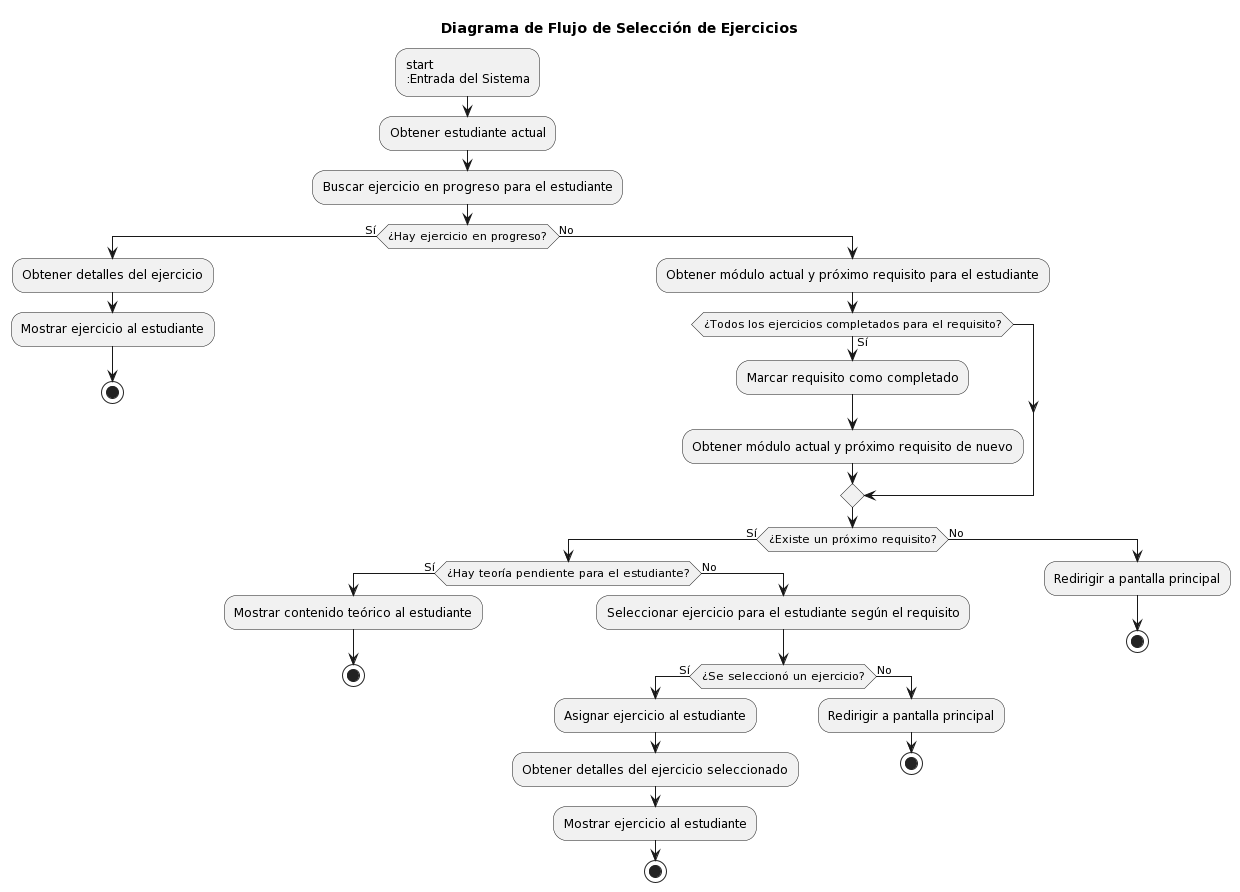
\includegraphics[width=\textwidth]{imagenes/seleccionejercicios.png}
\caption{Diagrama de flujo para la selección de ejercicios}
\label{fig:seleccion}
\end{figure}

\subsection{Cálculo del Tiempo para un Ejercicio}

Para calcular el tiempo estimado que un estudiante debe dedicar a un ejercicio, el sistema implementa un algoritmo adaptativo que considera tanto el historial de aprendizaje como la edad del estudiante (véase figura \ref{fig:calculotiempo}) . Este proceso se divide en dos etapas principales:


\paragraph{Obtención del Promedio de Tiempos}: El sistema calcula el tiempo promedio invertido por el estudiante en los últimos ejercicios. Matemáticamente, esto se representa como:

\begin{equation} 
    \text{promedio\_tiempos} = \frac{1}{n} \sum_{i=1}^{n} \text{tiempo\_i}
\end{equation}
    
donde \texttt{n} es el número de ejercicios considerados y \texttt{tiempo\_i} es el tiempo gastado en el i-ésimo ejercicio.

\paragraph{Ajuste del Tiempo Basado en la Edad}: Con el promedio obtenido, el sistema realiza un ajuste basado en la edad del estudiante para establecer un tiempo límite personalizado. 

\begin{equation}
    \begin{split}
        \text{tiempo\_limite} = \max\Bigg( & \text{t\_minimo}, \\
        & \left( \text{t\_maximo} - \text{ajuste\_edad} \right) \times \text{ponderacion\_edad} \\
        & + \left( \text{promedio\_tiempos} \times \text{ponderacion\_promedio} \right) \Bigg)
    \end{split}
\end{equation}
    
donde se da más importancia a la ponderación basada en la edad (80\%) que en el promedio de los tiempos anteriores (20\%). Asimismo, el tiempo mínimo para la realización de un ejercicio son 10 minutos, y el máximo unos 30 minutos. )

El resultado final es una estimación del tiempo que el estudiante debería dedicar a un nuevo ejercicio, asegurando que los ejercicios sean adecuados a su nivel de habilidad y ritmo de aprendizaje. De esta manera se consigue promover un entorno de aprendizaje equilibrado y efectivo, adaptándose a las necesidades individuales de cada estudiante.

\begin{figure}[H]
\centering
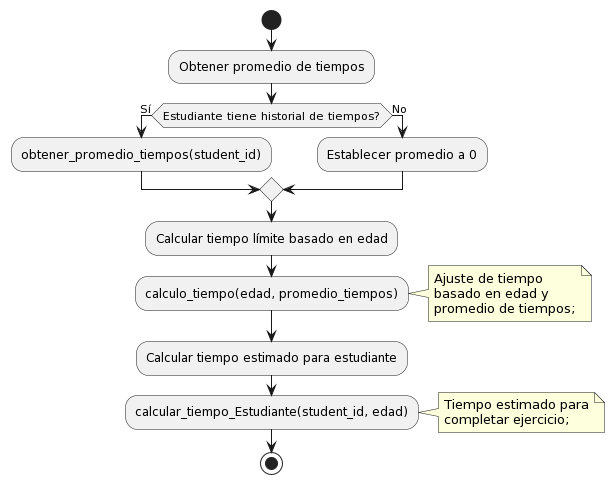
\includegraphics[width=0.8\textwidth]{imagenes/calculotiempo.png}
\caption{Diagrama de flujo para el cálculo del tiempo de un ejercicio}
\label{fig:calculotiempo}
\end{figure}

\subsection{Corrección y evaluación de calidad del código}

El verdadero reto comienza tras la entrega de un ejercicio por parte del estudiante. La lógica de corrección evalúa el código en términos de precisión y calidad. Si un código no alcanza un estándar mínimo, el sistema propone ejercicios adicionales, reforzando así las áreas de mejora del estudiante (véase figura \ref{fig:correccion}) . La justificación detrás de esta lógica se centra en la premisa de que la repetición y el refuerzo son esenciales para consolidar el aprendizaje. Además, al establecer estándares de calidad, se fomentan las buenas prácticas de programación desde las etapas iniciales de formación.

\begin{figure}[H]
    \centering
    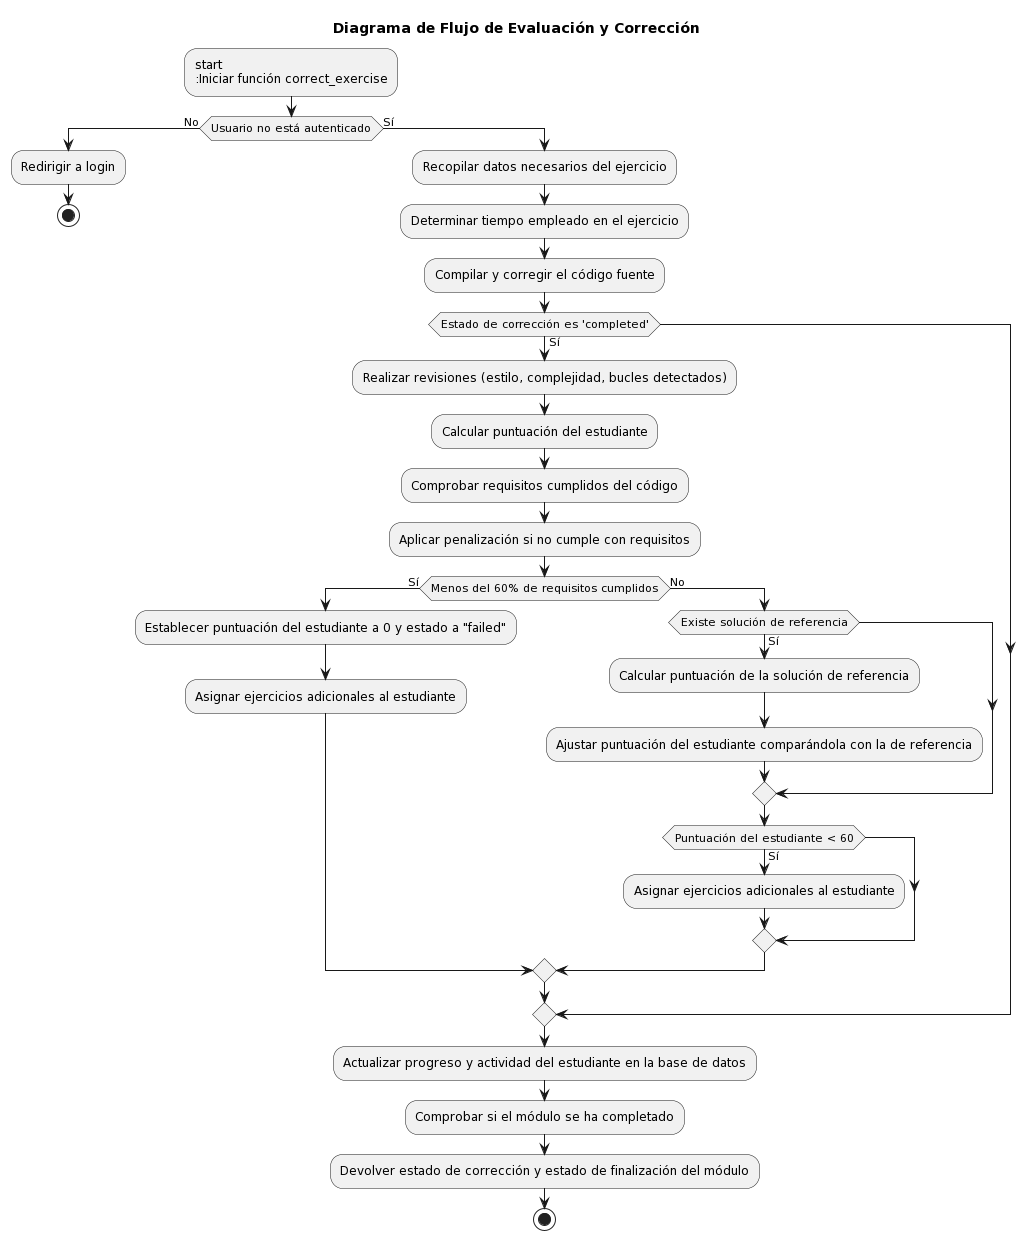
\includegraphics[width=\textwidth]{imagenes/correcionejercicios.png}
    \caption{Diagrama de flujo para la corrección de ejercicios}
    \label{fig:correccion}
\end{figure}

\subsection{Comprobaciones del código}

Una de las partes más importantes de la corrección es la comprobación de la calidad del código en diversos ámbitos. 

\subsubsection*{Evaluación del estilo del código}

El estilo del código es un aspecto crítico que influye directamente en su legibilidad, mantenibilidad y coherencia. Para garantizar la adherencia a las normas de estilo establecidas y promover prácticas de codificación de alta calidad, se implementan procedimientos de evaluación específicos para cada lenguaje de programación.

\begin{itemize}
    \item \textbf{Python}: En este caso, se usa \textit{pylint}, una herramienta de análisis estático ampliamente reconocida por su exhaustividad en la evaluación del estilo y calidad del código Python. \textit{pylint} no solo detecta errores y problemas de estilo, sino que también sugiere mejoras y refactoring para optimizar el código.

    \item \textbf{Java}: Se elige \textit{checkstyle}, una herramienta especializada en la conformidad con las convenciones de codificación de Java. Su capacidad para configurar y personalizar reglas la hace ideal para adaptarse a diferentes estilos y prácticas de codificación en Java. Concretamente, se han seguido las directrices de una de las configuraciones más usadas, \texttt{google-checks.xml}.

    \item \textbf{C++}: Para C++, se opta por \textit{cpplint}, una herramienta que se alinea con las directrices de Google para la codificación en C++. \textit{cpplint} examina el código fuente de C++ para identificar patrones que no se ajustan a las prácticas de codificación recomendadas, asegurando así un código limpio y bien estructurado.
\end{itemize}

\subsubsection*{Cálculo de la Complejidad Ciclomática}

La complejidad ciclomática, que mide el número de caminos de ejecución independientes en el código, es un indicador crucial de la complejidad y posibles riesgos asociados con el mantenimiento del código.

\begin{equation}
    V(G) = E - N + 2P
\end{equation}

donde: \\ \\
    V(G) es la complejidad ciclomática del programa. \\
    E representa el número de aristas en el grafo de flujo de control. \\
    N es el número de nodos en el grafo de flujo de control.\\
    P es el número de componentes conexos del grafo (generalmente P=1 en programas secuenciales).\\

Para los tres lenguajes, se ha usado \textit{Lizard}, una herramienta versátil de análisis de código que soporta múltiples lenguajes. Además, \textit{Lizard} no solo calcula la complejidad ciclomática, sino que también proporciona métricas detalladas sobre la longitud de las funciones y la cantidad de parámetros, ofreciendo así una visión integral de la complejidad del código

\subsubsection*{Detección de Bucles Infinitos}
Detectar y mitigar la presencia de bucles infinitos es esencial para asegurar la finalización adecuada de los programas y prevenir el consumo excesivo de recursos.

Para la detección de bucles infinitos en estos lenguajes, se implementó un sistema de ejecución controlada con temporizadores \ref{fig:comprobaciones}. Este método implica la ejecución del código en un entorno controlado, monitorizando el tiempo de ejecución. Si el código excede un tiempo límite predefinido, se interrumpe la ejecución, indicando la presencia potencial de un bucle infinito. Este enfoque es efectivo en la identificación de problemas de control de flujo que podrían no ser evidentes durante la inspección de código estático. Aunque cabe destacar que su efectividad no es tan alta como las anteriores comprobaciones. 

\begin{figure}[H]
    \centering
    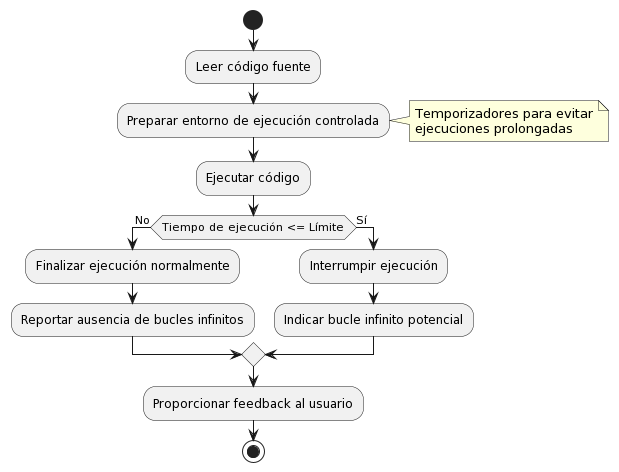
\includegraphics[width=0.8\textwidth]{imagenes/buclesinfinitos.png}
    \caption{Diagrama de flujo para la comprobación de bucles infinitos}
    \label{fig:comprobaciones}
\end{figure}

\subsection{Comprobación del cumplimiento de los requisitos}

Verificar el cumplimiento de requisitos específicos es fundamental para asegurar la calidad y la adecuación del código a ciertos estándares y objetivos pedagógicos. Para realizar esta tarea de manera eficaz, se han desarrollado clases especializadas que analizan el Árbol de Sintaxis Abstracta (AST) \cite{astlibrary} del código. Estas clases, adaptadas para cada lenguaje de programación principal, permiten una inspección detallada y específica del código fuente.

\subsubsection*{Comprobación en Python}

Para Python, la clase \texttt{RequirementVisitor}, que extiende de \texttt{ast.Node Visitor}, es la encargada de esta tarea. Mediante la inicialización de un diccionario \texttt{requirements\_found}, esta clase mapea una serie de conceptos clave (como operadores básicos y lógicos, estructuras de control, funciones y clases) a valores booleanos. A través de métodos como \texttt{visit\_BinOp}, \texttt{visit\_If} y \texttt{visit\_ClassDef}, la clase examina el AST en busca de estos elementos, marcando cada requisito encontrado como verdadero  (véase figura \ref{fig:arbolrequisios}).

\subsubsection*{Comprobación en Java}

En el caso de Java, la clase \texttt{RequirementVisitor\_JAVA} adopta un enfoque similar. Utilizando el analizador \textit{javalang}, esta clase recorre el AST del código Java, identificando estructuras tales como operaciones binarias, declaraciones \textit{if-else}, bucles y definiciones de métodos y clases. La detección de estos elementos actualiza el estado de los requisitos en el diccionario correspondiente.

\subsubsection*{Comprobación en C++}

Para C++, se utiliza la clase \texttt{RequirementVisitor\_CPP}, que aprovecha las capacidades de la biblioteca \textit{clang} para analizar el AST. Esta clase, al igual que sus contrapartes en Python y Java, busca patrones específicos en el código, tales como operadores, estructuras de control y definiciones de clases y funciones, actualizando su registro de requisitos encontrados.

Independientemente del lenguaje, el proceso comienza con la lectura y el análisis del código fuente para generar el AST correspondiente. Posteriormente, se instancia la clase visitante apropiada y se recorre el árbol, actualizando el estado de los requisitos encontrados. Esta metodología asegura una evaluación detallada y uniforme del cumplimiento de requisitos en diferentes lenguajes de programación. A continuación, se muestra el diagrama de flujo para la comprobación de requisitos en Python. Notése que el diagrama es analogo para los otros dos lenguajes de programación.


\begin{figure}[H]
    \centering
    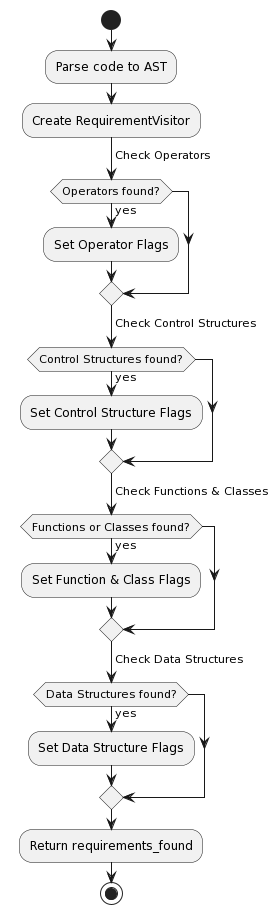
\includegraphics[width=0.3\textwidth]{imagenes/comprobacionescodigo.png}
    \caption{Diagrama de flujo que ilustra cómo se comprueban los requisitos dentro del árbol para Python}
    \label{fig:arbolrequisios}
\end{figure}


\subsection{Cálculo de la puntuación}

El sistema utiliza la función \texttt{calculate\_score} para calcular la puntuación de un ejercicio. Esta función combina múltiples criterios que inciden en la calidad y eficacia del código del estudiante (véase figura \ref{fig:puntuacion}).

\begin{itemize}
    \item \textbf{Problemas de Estilo}: Detectados mediante un análisis estático. Cada inconveniente identificado resta 5 puntos de los 100 iniciales.
    
    \item \textbf{Complejidad Ciclomática}: Un valor elevado (superior a 10) en la complejidad ciclomática suele indicar que el código puede ser difícil de mantener o probar. Por ello, se aplica una penalización significativa de 20 puntos. Esta cantidad ha sido establecida para subrayar la importancia de escribir código sencillo y fácilmente comprensible.
        
    \item \textbf{Bucles Detectados}: La presencia de bucles no es necesariamente un problema, pero puede llevar a un código menos eficiente o más complejo si no se usan adecuadamente. Se resta una cantidad menor, 15 puntos, con tal de incentivar el uso cuidadoso de estas estructuras.    
\end{itemize}

La fórmula que resume todo el proceso es la siguiente:

\begin{equation}
\max \left( 0, 100 - 5 \times \text{Problemas de Estilo} - 20 \times I_{\text{complejidad > 10}} - 15 \times I_{\text{bucles detectados}} \right)
\end{equation}

Cabe destacar que $I_{\text{condición}}$ actúa como una función indicadora. Toma el valor de 1 si la condición se cumple y 0 en caso contrario.

\begin{figure}[H]
    \centering
    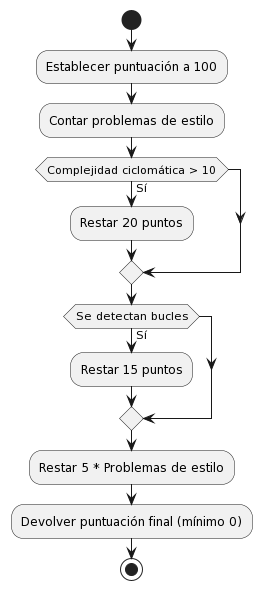
\includegraphics[width=0.3\textwidth]{imagenes/puntuacionejercicio.png}
    \caption{Diagrama de flujo que ilustra cómo se calcula la puntuación}
    \label{fig:puntuacion}
\end{figure}

Finalmente, la función tiene un control para que la puntuación no sea negativa, con tal de evitar la desmotivación del estudiante. Devuelve el máximo entre el valor calculado y cero.

\subsection{Cálculo del número extra de ejercicios}

El principal objetivo de la función \texttt{determine\_number\_of\_extra\_exercises} es adaptar de manera dinámica la carga de ejercicios asignados a un estudiante en función de su desempeño reciente, ofreciendo una experiencia de aprendizaje más personalizada (véase figura \ref{fig:numextraejercicios}) .

\subsubsection{Parámetros de Entrada}

La función acepta los siguientes argumentos:

\begin{itemize}
    \item \textbf{student\_id}: Este identificador único del estudiante se utiliza para acceder a sus registros y recuperar su historial de rendimiento.
    \item \textbf{recent\_num = 4}: Este parámetro establece que se tendrán en cuenta los últimos 4 ejercicios completados para evaluar la tasa de fracaso del estudiante. El número 4 se ha seleccionado como un equilibrio entre tener una muestra lo suficientemente grande para ser significativa, pero no tan grande como para ser desactualizada.
    \item \textbf{max\_extra\_exercises = 5}: Este es el número máximo de ejercicios adicionales que se pueden asignar. Limitar esto a 5 ayuda a prevenir una carga de trabajo abrumadora y repetitiva para el estudiante.
    \item \textbf{failure\_rate\_threshold = 0.35}: Se asignarán ejercicios adicionales si la tasa de fracaso supera este umbral. El valor de 0.35 se establece para permitir cierto margen de error pero todavía requiere una intervención si el rendimiento del estudiante es consistentemente bajo.
\end{itemize}

\subsubsection{Flujo de Trabajo y Razonamiento}

El flujo de trabajo de la función se puede desglosar en las siguientes etapas:

\begin{enumerate}
    \item \textbf{Consulta de Requisitos}: La función primero identifica el último ``requisito'' completado por el estudiante para determinar desde dónde empezar.
    \item \textbf{Búsqueda de Ejercicios Relacionados}: Se recuperan los IDs de los ejercicios asociados con el requisito actual para tener un conjunto de datos sobre el cual operar.
    \item \textbf{Recolección y Análisis de Datos}: A continuación, se evalúa el rendimiento del estudiante en estos ejercicios, especialmente en términos de fracasos y éxitos, para calcular una tasa de fracaso.
    \item \textbf{Normalización del Tiempo Empleado}: Los tiempos empleados en los ejercicios se normalizan para darles una escala uniforme, lo que permite una mejor comparación.
    \item \textbf{Ponderación y Cálculo Final}: Los dos factores (tasa de fracaso y tiempo normalizado) se combinan en una suma ponderada para determinar el número final de ejercicios extra.
\end{enumerate}

La fórmula utilizada para calcular el número de ejercicios extra es la siguiente:

\begin{equation}
N = \max\left(0, \text{round}\left( w_f \times f + w_t \times t \right) \times M \right)
\end{equation}

Donde:

\begin{itemize}
    \item \( w_f = 0.7 \) y \( w_t = 0.3 \) son los pesos asignados a la tasa de fracaso y al tiempo, respectivamente. Estos pesos reflejan la importancia relativa de cada factor; en este caso, la tasa de fracaso se considera más crítica.
    \item \( f \) es la tasa de fracaso actual del estudiante.
    \item \( t \) es el tiempo normalizado del último ejercicio.
    \item \( M \) es el número máximo de ejercicios extra permitidos.
\end{itemize}

\begin{figure}[H]
    \centering
    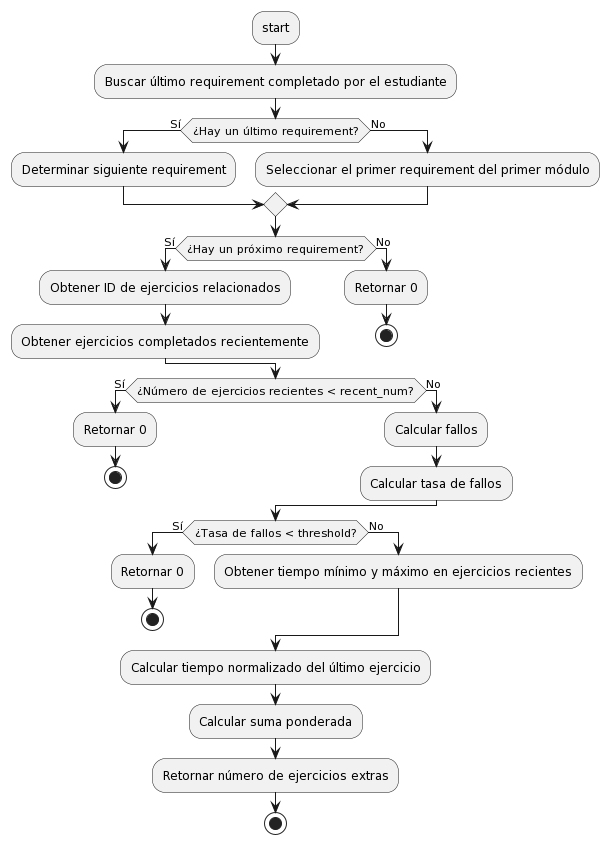
\includegraphics[width=0.6\textwidth]{imagenes/numeroejersextras.png}
    \caption{Diagrama de flujo que ilustra el cálculo del número extra de ejercicios}
    \label{fig:numextraejercicios}
\end{figure}

\section{Implementación de Módulos de Aprendizaje Adaptativo}

El núcleo de nuestro sistema educativo se centra en un modelo de aprendizaje adaptativo, diseñado para responder de manera dinámica al progreso y las necesidades del estudiante. La idea es no solo adaptar el tipo de material de aprendizaje presentado, sino también ajustar la cantidad y complejidad de los ejercicios asignados, todo en tiempo real.

La adaptación del sistema se logra mediante una combinación de técnicas de análisis de datos. En primer lugar, se recopilan métricas clave del rendimiento del estudiante, como las tasas de éxito y fracaso en ejercicio, o el tiempo empleado. Estos datos se almacenan y analizan para determinar patrones y tendencias que luego son utilizadas para tomar decisiones adaptativas.

En el nivel más básico, el sistema cuenta con un conjunto predefinido de requisitos de aprendizaje, que son objetivos educativos específicos que el estudiante debe alcanzar. A medida que el estudiante avanza, el sistema evalúa continuamente su rendimiento y ajusta los requisitos de aprendizaje en función de este. Por ejemplo, si un estudiante supera con facilidad los ejercicios iniciales en un tema, el sistema puede decidir si avanzarle a un nuevo tema más rápidamente.

Además, en situaciones donde un estudiante demuestra dificultades persistentes, como una tasa de fracaso elevada en ejercicios recientes, el sistema asigna automáticamente ejercicios adicionales de refuerzo con tal ayudar al estudiante a mejorar en las áreas problemáticas, como se detalla en la sección anterior sobre el cálculo del número extra de ejercicios.

Un aspecto crítico que distingue esta implementación es la adaptabilidad basada en una solución de referencia proporcionada por el profesor. Este enfoque mitiga cualquier rigidez en el proceso de evaluación y garantiza que la retroalimentación sea contextual y ajustada. 

El ajuste de la puntuación del estudiante se realiza mediante las siguientes fórmulas para calcular el fitness y la puntuación respectivamente:

\begin{equation}
\max\left(0, 1 - \frac{| \text{teacher\_score} - \text{student\_score} |}{100} \right)
\end{equation}

\begin{equation}
\text{student\_score} \times= \text{fitness}
\end{equation}

La variable \texttt{fitness} calcula la discrepancia entre la puntuación del estudiante y la del profesor. Este valor luego multiplica la puntuación original del estudiante para ajustarla. 

En resumen, la implementación de módulos de aprendizaje adaptativo en el sistema se lleva a cabo a través de un análisis cuidadoso de los datos del rendimiento del estudiante, seguido de la toma de decisiones algorítmicas para personalizar la experiencia de aprendizaje. Esta aproximación permite no solo una mayor eficiencia en el proceso educativo, sino también una experiencia más personalizada y, por ende, más atractiva para el estudiante.

